%                                                                 aa.dem
% AA vers. 8.3, LaTeX class for Astronomy & Astrophysics
% demonstration file
%                                                       (c) EDP Sciences
%-----------------------------------------------------------------------

\documentclass{aa}
%\documentclass[referee]{aa}        % for a referee version
%\documentclass[onecolumn]{aa}      % for a paper on 1 column
%\documentclass[longauth]{aa}       % for the long lists of affiliations
%\documentclass[rnote]{aa}          % for the research notes
%\documentclass[letter]{aa}         % for the letters
%\documentclass[bibyear]{aa}        % if the references are not structured
                                    % according to the author-year
                                    % natbib style

%%%%%%%%%%%%%%%%%%%%%%%%%%%%%%%%%%%%%%%%
\usepackage{natbib}
\usepackage{graphicx}
\usepackage{txfonts}
\usepackage{hyperref}
\hypersetup{
    colorlinks=true,   %% links colored instead of frames
    urlcolor=blue,     %% external hyperlinks
    linkcolor=red,     %% internal latex links (eg Fig)
    citecolor=blue,
}
%%%%%%%%%%%%%%%%%%%%%%%%%%%%%%%%%%%%%%%%
% To add links in your PDF file, use the package "hyperref"
% with options according to your LaTeX or PDFLaTeX drivers.

\begin{document}
  \title{Comparison of multi-frequency positions of extra-galactic sources}
%   \subtitle{I. Overviewing the $\kappa$-mechanism}
  \author{N. Liu\inst{1}
     \and
          S. B. Lambert\inst{2}\fnmsep
          \and
          C.-Y. Ding\inst{1}
          \and
          N. Jiang\inst{1}
          \and
          Z. Zhu\inst{1}
          \and
          J.-C. Liu\inst{1}
        %   \thanks{Just to show the usage of the elements in the author field}
          }

  \institute{School of Astronomy and Space Science,
   		     Key Laboratory of Modern Astronomy and Astrophysics (Ministry of Education), Nanjing University, Nanjing, P. R. China\\
              \email{liuniu@smail.nju.edu.cn;zhuzi@nju.edu.cn}
         \and
             SYRTE, Observatoire de Paris,
             Universit\'e PSL, CNRS, Sorbonne Universit\'e, LNE, Paris, France\\
             \email{sebastien.lambert@obspm.fr}
            %  \thanks{The university of heaven temporarily does not
                    %  accept e-mails}
             }

  \date{Received; accepted}


  \abstract
  % context heading (optional)
  % {} leave it empty if necessary
   {
       Previous comparisons of the \textit{Gaia} and radio positions measured by the very long baseline interferometry (VLBI) at $X$-band probe the structure of the milli-arcsecond (mas) scale of Active Galactic Nucleus.
       But the available VLBI positions at high frequencies are less tapped.
   }
  % aims heading (mandatory)
   {
       We aim to study the multi-frequency position of extra-galactic sources, complementary to previous studies.}
  % methods heading (mandatory)
   {
       We compared the absolute positions measured at four different bands,
       that is, optical position from the {\it Gaia} Data Release 2 and three radio positions at $X$-, $K$-, and $Ka$-band from the ICRF3 catalog, for 488 common sources.
       We first aligned the $K$-band, $Ka$-band, and \textit{Gaia} catalogs onto the $X$-band frame.
       Then we studied the frequency-position relation and correlation of radio-to-optical offsets determined at different radio bands
       with the magnitude, source morphological properties, and relativistic jet properties.
   }
  % results heading (mandatory)
   {
       The deviation amongst radio-to-optical offsets at different radio bands is less than 0.5~mas for 91\% of the sample.
       The large radio-to-optical offset appears to favor faint quasars but are well accounted for by their error.
       We found that the $K$-band, $Ka$-band, and \textit{Gaia} positions are on the same side of the $X$-band that is, four-band positions aligned, for 47 cases.
       However, this position-alignment relation is vulnerable to the global systematics.
       For these sources with four-band positions aligned and also with available jet direction determination, more than half of them have a radio-to-optical offset parallel to the jet.
       %A simulation considering the position error ellipses suggests that four positions of extra-galactic objects agree at a level of 0.1~mas.
       %, even though small offsets could be obtained from the given positions in catalogs
   }
  % conclusions heading (optional), leave it empty if necessary
   {
       The source structure might not affect the radio source position at $X$-band much
       The selection of sources for link between the ICRF and \textit{Gaia}-CRF is not neccessarily limited to bright quasars only.
       %The selection criteria of optically bright radio-loud sources for frame-link at $X$-band might also work for the $K$- and $Ka$-band.
       Our results also justify the reliability of the ICRF3 $X$-band frame.
   }

  \keywords{techniques: interferometric --
            astrometry --
            quasars: general}

\maketitle

%________________________________________________________________

\section{Introduction}     \label{sec:introduction}

   The frequency-dependent position of extragalactic objects (mostly distant quasars) is of interest in both astrometric and astrophysical fields, especially the position offset between the optical centroid and radio core.
   Such studies can be used to maintain and improve the celestial reference frames materialized by positions of extragalactic objects.
   For example, the optical observations of the ICRF2 sources in the Rio survey monitors the frame-link status between the \textit{Hipparcos} celestial reference frame and the International Celestial Reference Frame (ICRF) \citep{2013MNRAS.430.2797A}.
   The study of radio-to-optical offset also provides a probing of the structure properties of Active Galactic Nucleus (AGNs), such as the accretion disc and relativistic jet \citep[e.g.,][]{2019ApJ...871..143P}.

   Accurate positions at sub-milli-arcsecond (mas) are needed for studying the frequency-position relation, which were achieved exclusively by the very long baseline interferometry (VLBI).
   The arrival of \textit{Gaia} Data release 2 \citep[\textit{Gaia} DR2;][]{2016A&A...595A...1G,2018A&A...616A...1G} data provides optical positions of quasars with a precision close to their VLBI positions.
   The comparison between \textit{Gaia} and VLBI positions measured at 8~GHz shows excellent agreements on the level of 1~mas except about 6\%-9\% of outliers, that is, significant \textit{Gaia}/VLBI offsets \citep{2016A&A...595A...5M,2018A&A...616A..14G,2017MNRAS.471.3775P,2017MNRAS.467L..71P,2017A&A...598L...1K,2017ApJ...835L..30M,2018AJ....155..229F,2019MNRAS.482.3023P,2019ApJ...871..143P,2020MNRAS.493L..54K}.
   Recently, \citet{2019MNRAS.482.3023P} report that for 62\% of sources with a significant \textit{Gaia}/VLBI offset and also a determinable jet direction, the VLBI-to-\textit{Gaia} offset vector is parallel to the jet.
   \citet{2019ApJ...871..143P,2020MNRAS.493L..54K} further extend this study and find a correlation between the \textit{Gaia}/VLBI offset parallel to jet direction with the dominance of different AGN component in the optical emission, AGN classifications, and optical polarization properties.

   These studies, however, are only limited to the VLBI positions at $X$-band.
   Note that VLBI positions at higher frequencies, such as $K$- and $Ka$-band, are also feasible, which show competing precisions to that of $X$-band \citep[e.g.,][]{2019evga.confP.302J,2019evga.confP.306D}.
   The $K$- and $Ka$-band positions suffer less from the radio source structure and ionosphere and solar plasma effects than those at $X$-band \citep[e.g.,][]{2002ivsg.conf..350J}.
   Including $K$- and $Ka$-band positions in the \textit{Gaia}/VLBI offset studies would help understand the origin of the radio-to-optical offsets.
   On the other side, the link between $K$- and $Ka$-band VLBI frames and the \textit{Gaia} celestial reference frame (\textit{Gaia}-CRF) also requires detailed studies on the position offsets between $K$- and $Ka$-band and \textit{Gaia}.

   We aim to compare the multi-frequency positions of extra-galactic sources, in order to complement findings led by \citet{2019MNRAS.482.3023P}.
   We computed the \textit{Gaia}/VLBI offsets at $X$-, $K$-, and $Ka$-band and studied their dependency on the properties of AGNs, such as the magnitude, redshift, source structure at radio and optical domain.
   These comparisons are intended to provide new insights to understanding of the origin of radio-to-optical offset, as well as the link between \textit{Gaia}-CRF and VLBI frames other than $X$-band.

%__________________________________________________________________

\section{Data and methods}    \label{sec:obs}

%__________________________________________________ {tab:median-err}
    \begin{table}[htbp]
        \centering
        \caption{\label{tab:median-err}
            Fromal uncertainty for 488 common sources amongst ICRF3 $X$-band, $K$-band, $Ka$-band, and \textit{Gaia}-CRF2 catalogs.
        }
        \begin{tabular}{cccc}
            \hline \noalign{\smallskip}
            Catalog &$\sigma_\alpha\cos\delta$  &$\sigma_\delta$  &$\sigma_{\rm pos,max}$\\
            & $\mathrm{\mu as}$ & $\mathrm{\mu as}$  & $\mathrm{\mu as}$ \\
            \noalign{\smallskip}
            \hline
            \noalign{\smallskip}
            ICRF3 $X$      & 43  & 53  & 55  \\
            ICRF3 $K$      & 66  &126  &128  \\
            ICRF3 $Ka$     & 67  & 98  &104  \\
            \textit{Gaia}  &189  &167  &218 \\
            \hline
        \end{tabular}
        \tablefoot{$\sigma_{\rm pos,max}$ represents the semi-major axis of the error ellipse.
        }
    \end{table}

   We used the radio positions of quasars measured by VLBI at $X$-, $K$-, and $Ka$-band from the ICRF3 catalog publicly available at the Paris Observatory IERS ICRS Center\footnote{\url{http://hpiers.obspm.fr/icrs-pc/newwww/icrf/index.php}}.
   For positions of their optical counterparts, we took the ICRF3-prototype sample (\texttt{gaiadr2.aux\_iers\_gdr2\_cross\_id} table) from the \textit{Gaia}-DR2 archive\footnote{\url{http://gea.esac.esa.int/archive/}}.
   The cross-match amongst these four catalogs gave a list of 488 common sources.

   % The median formal uncertainties on the right ascension, declination, and along the semi-major axis of error ellipse are $\mathrm{43\,\mu as}$, $\mathrm{53\,\mu as}$, and $\mathrm{55\,\mu as}$, respectively, for the $X$-band positions.
   % The corresponding values are $\mathrm{66\,\mu as}$, $\mathrm{126\,\mu as}$, and $\mathrm{128\,\mu as}$ for their $K$-band positions;
   % $\mathrm{67\,\mu as}$, $\mathrm{98\,\mu as}$, and $\mathrm{104\,\mu as}$ at $Ka$-band;
   % and $\mathrm{189\,\mu as}$, $\mathrm{167\,\mu as}$, and $\mathrm{218\,\mu as}$ for \textit{Gaia} positions.
   % Therefore, the $X$-band position precision is generally twice better than the $K$- and $Ka$-band, and nearly four times better than the \textit{Gaia} DR2 positions for the sample used here.
   % This frequency-error relation differs from that the VLBI formal uncertainty decreases with the observing frequency, which is obtained using all sources in each catalogs \citep{2020A&A...634A..28L}.
   The median formal uncertainties on the right ascension, declination, and along the semi-major axis of error ellipse in four catalogs are given in Table~\ref{tab:median-err}.
   For the sample used here, the $X$-band position precision is generally twice better than the $K$- and $Ka$-band, and nearly four times better than the \textit{Gaia} DR2 positions.
   This frequency-error relation differs from that the VLBI formal uncertainty decreases with the observing frequency, which is obtained using all sources in each catalogs \citep{2020A&A...634A..28L}.

   Even the ICRF3 and the \textit{Gaia}-CRF2 are both the realizations of the International Celestial Reference System \citep[ICRS;][]{1995A&A...303..604A,1998A&A...331L..33F}, \citet{2020A&A...634A..28L} have revealed some zonal (declination-dependent) errors as large as 0.2~mas in the $Ka$-band frame, which might bias our analyses here.
   In order to model and, subsequently, remove these systematical differences, we used the vector spherical harmonics \citep[VSH;][]{2012A&A...547A..59M} of degree 2, whose equation could be found in \citet[][their Eq.~(1)]{2020A&A...634A..28L}.
   We followed similar procedures described therein to determine 16 transformation parameters between celestial reference frames at different wavelengths.
   The $X$-band celestial frame was chosen as the reference frame since it is the most precise celestial reference frame so far.
   In addition, it is the fundamental frame and has a long history.
   By doing so, we permit to analyze multi-wavelength positions in a consist celestial frame and avoid possible bias arising from the alignment and deformation of the celestial reference frames.

   We then measured three radio-to-optical offsets, that is, the angular separation $\rho$ between $X$-, $K$-, and $Ka$-band and \textit{Gaia} positions.
   We also computed the normalized separation $X$ following the same precedures in the \citet[][their X-statistics]{2016A&A...595A...5M},
   to account for the formal uncertainty and correlation between right ascension and declination of individual sources.
   These two quantities serve as indicators of significant radio-to-optical offset as done in recent works \citep[e.g.,][]{2019MNRAS.482.3023P,2018A&A...616A..14G}.

   The correlations between radio-to-optical distances and source properties were analyzed by statistical tests, namely, the Pearson correlation test (parametric test) and the Spearman and the Kendall rank-correlation tests (non-parametric test).
   \citet{2013MNRAS.430.2797A} adopt these methods on a similar topics (Their optical positions were obtained from ground-based observations).

   In order to study the influence of \textit{Gaia} formal uncertainty on the radio-to-optical distances, we correlated the radio-to-optical offsets with $G$ magnitude given in the {\it Gaia} DR2 catalogs.
   As the \textit{Gaia} formal uncertainty becomes worse for fainter objects, the selection of frame-tie objects for the ICRF and \textit{Gaia}-CRF prefers optically bright quasars \citep[visual magnitude $V<17$, see, e.g.,][]{2008A&A...490..403B}.

   Besides, we considered the source morphological properties in both optical and radio domains, characterized by (optical) morphological indices (MIs) from the fifth release of the Large Quasar Astrometric Catalogue \citep[LQAC-5;][]{2019A&A...624A.145S} and the structure index \citep[SI;][]{1997ApJS..111...95F} at $X$-band from the Bordeaux VLBI Imaging database (BVID) \footnote{\url{http://bvid.astrophy.u-bordeaux.fr/}}.
   The morphological indices were derived from the $B$, $R$,  and $IR$  DSS (Digital Sky Survey) images.
   Three indices are given for each plates, which are SHARP, SROUND, and GROUND index probing skewness, roundness, and normalness of the quasar point spread function, respectively.
   The structure index emerges clearly from snapshot and might be strongly epoch-dependent, therefore, we only used structure indices from images made between J2014 and J2016, within one year to the position reference epoch J2015 of the ICRF3 catalog.
   Our underlying assumption is that the structure of AGNs will not change significantly among one year, thus does the structure index.
   If more than one structure index are given for single sources (observations made more than one epoch), we used the one made as close as possible to J2015.

   The extend structure of extra-galactic objects might shift the optical position measured by \textit{Gaia}.
   However, this effect would be less significant for sources locating far away from us, that is, with a high redshift.
   Another perturbation on the optical position comes from the existence of host galaxy.
   In order to check these two effects, we included in our analyses the redshift $z$ taken from the LQAC-5 catalog as well.

   In order to study the relative positions of emission centers at different frequencies, we calculated the position angle (PA) of offsets of $K$-band, $Ka$-band, and \textit{Gaia} positions relative to the $X$-band position.
   The PA was counted as clockwise from the increasing direction of the declination axis.
   These position angles were compared with each one to check if they have any correlation, as well as the jet direction.
   % We also note that the formal uncertainty of source positions in the original catalogs might distort the determination of the PAs.
   % We performed a Monte-Carlo simulation to check our results.
   The jet direction of AGNs was retrieved the of Active Galactic Nucleus from the MOJAVE (Monitoring Of Jets in Active galactic nuclei with VLBA Experiments) survey \footnote{\url{http://www.physics.purdue.edu/astro/MOJAVE/index.html}} \citep[][]{2019ApJ...874...43L}.
   Note that the positions of jet features and might be epoch-dependent and so do their position angles referred to the compact core, we used the directions of linear motion of brightest ejecting jet features instead of their positions.
   % The same issue would occur to the images too, therefore, we only used the image made closest to J2015.
%   As illustrated in Fig.~\ref{fig:illustration-diagram},

%__________________________________________________________________

\section{Results}    \label{sec:result}

%__________________________________________________________________

\subsection{Removal of large-scale differences}    \label{subsec:remove-sys}

    %
    %__________________________________________________ {tab:vsh01}
    \begin{table*}[htbp]
        \centering
        \caption{\label{tab:vsh01}
            Rotation and glide and their formal uncertainties of ICRF3 $K$-band, $Ka$-band, and \textit{Gaia}-CRF2 catalogs with respect to the ICRF3 $X$-band catalog.
        }
        \begin{tabular}{cccccccc}
            \hline \noalign{\smallskip}
            &No. Sources & $R_1$ & $R_2$ & $R_3$ & $D_1$ & $D_2$ & $D_3$ \\
            & & $\mathrm{\mu as}$ & $\mathrm{\mu as}$  & $\mathrm{\mu as}$ & $\mathrm{\mu as}$ & $\mathrm{\mu as}$& $\mathrm{\mu as}$ \\
            \noalign{\smallskip}
            \hline
            \noalign{\smallskip}
            $K - X$    & 462 &$   -4 \pm     9$  &$   -5 \pm     9$  &$   -3 \pm     5$  &$  -10 \pm     8$  &$   30 \pm     8$  &$   34 \pm     8$  \\
            $Ka - X$   & 284 &$  -24 \pm    11$  &$   -8 \pm    11$  &$    1 \pm     8$  &$    4 \pm    10$  &$   29 \pm     9$  &$ -242 \pm    12$ \\
            $Gaia - X$ & 386 &$  -36 \pm    13$  &$   32 \pm    13$  &$   -3 \pm    13$  &$    9 \pm    13$  &$   -2 \pm    14$  &$    6 \pm    12$ \\
            \hline
        \end{tabular}
    \end{table*}
    %
    %__________________________________________________ {tab:vsh02}
    \begin{table*}[htbp]
        \centering
        \caption{\label{tab:vsh02}
            Quadrupolar terms and their formal uncertainties of ICRF3 $K$-band, $Ka$-band, and \textit{Gaia}-CRF2 catalogs with respect to the ICRF3 $X$-band catalog.
        }
        \begin{tabular}{ccccccccccc}
            \hline \noalign{\smallskip}
            &$E_{22}^R$  &$E_{22}^I$  &$E_{21}^R$  &$E_{21}^I$  &$E_{20}$    &$M_{22}^R$  &$M_{22}^I$  &$M_{21}^R$  &$M_{21}^I$  &$M_{20}$    \\
            & $\mathrm{\mu as}$ & $\mathrm{\mu as}$  & $\mathrm{\mu as}$ & $\mathrm{\mu as}$ & $\mathrm{\mu as}$& $\mathrm{\mu as}$ & $\mathrm{\mu as}$ & $\mathrm{\mu as}$  & $\mathrm{\mu as}$ & $\mathrm{\mu as}$  \\
            \noalign{\smallskip}
            \hline
            \noalign{\smallskip}
            $K - X$      &$   -6 \pm     3$  &$   -7 \pm     3$  &$  -25 \pm     9$  &$  -38 \pm     9$  &$  -15 \pm    10$  &$    6 \pm     5$  &$   -5 \pm     5$  &$   11 \pm     9$  &$  -29 \pm     9$  &$  -33 \pm     6$ \\
            $Ka - X$  &$   -4 \pm     5$  &$    4 \pm     5$  &$   -8 \pm    11$  &$   20 \pm    12$  &$   49 \pm    15$  &$   -3 \pm     6$  &$    2 \pm     7$  &$   -4 \pm    10$  &$    7 \pm    11$  &$  155 \pm    11$ \\
            $Gaia - X$    &$   -7 \pm     9$  &$   -4 \pm     8$  &$  -23 \pm    16$  &$  -11 \pm    16$  &$   -5 \pm    15$  &$    2 \pm     8$  &$   -4 \pm     8$  &$  -37 \pm    17$  &$  -24 \pm    17$  &$  -11 \pm    15$ \\
            \hline\end{tabular}
    \end{table*}

    %
    %__________________________________________________  {fig:k-sx-pos-offset-scatter}
    \begin{figure}[hbtp]
        \centering
        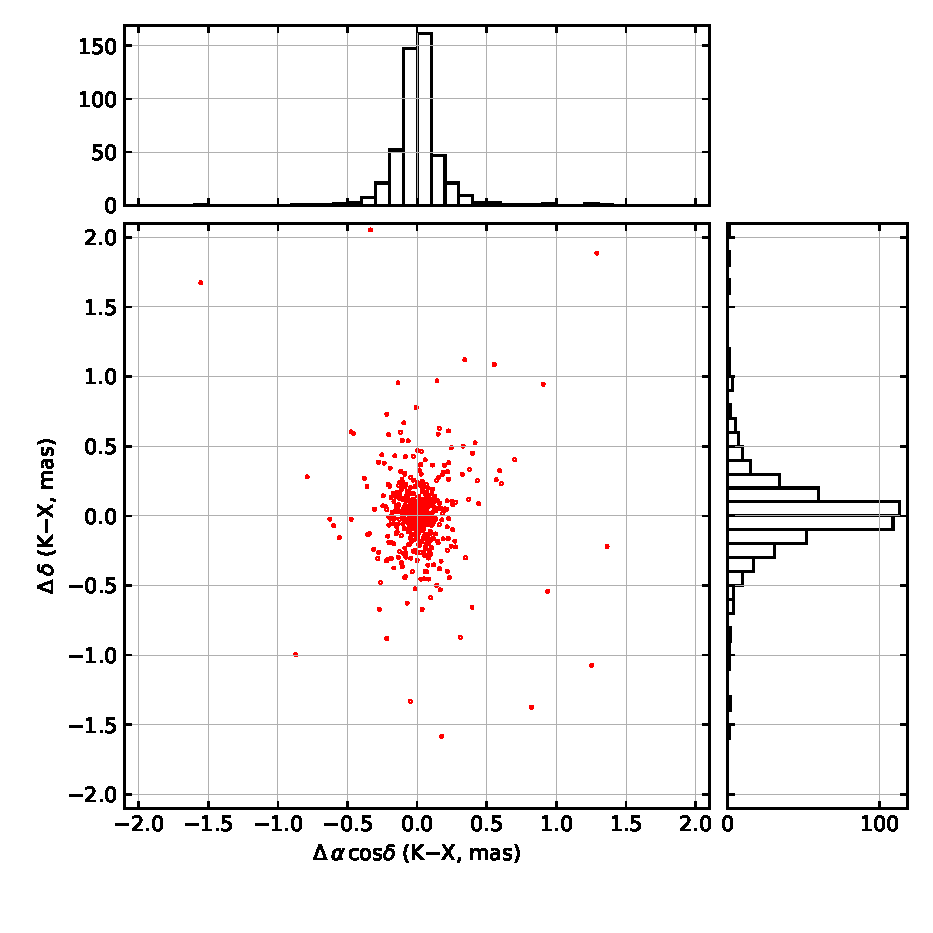
\includegraphics[width=60mm]{figs/k-sx-scatter}
        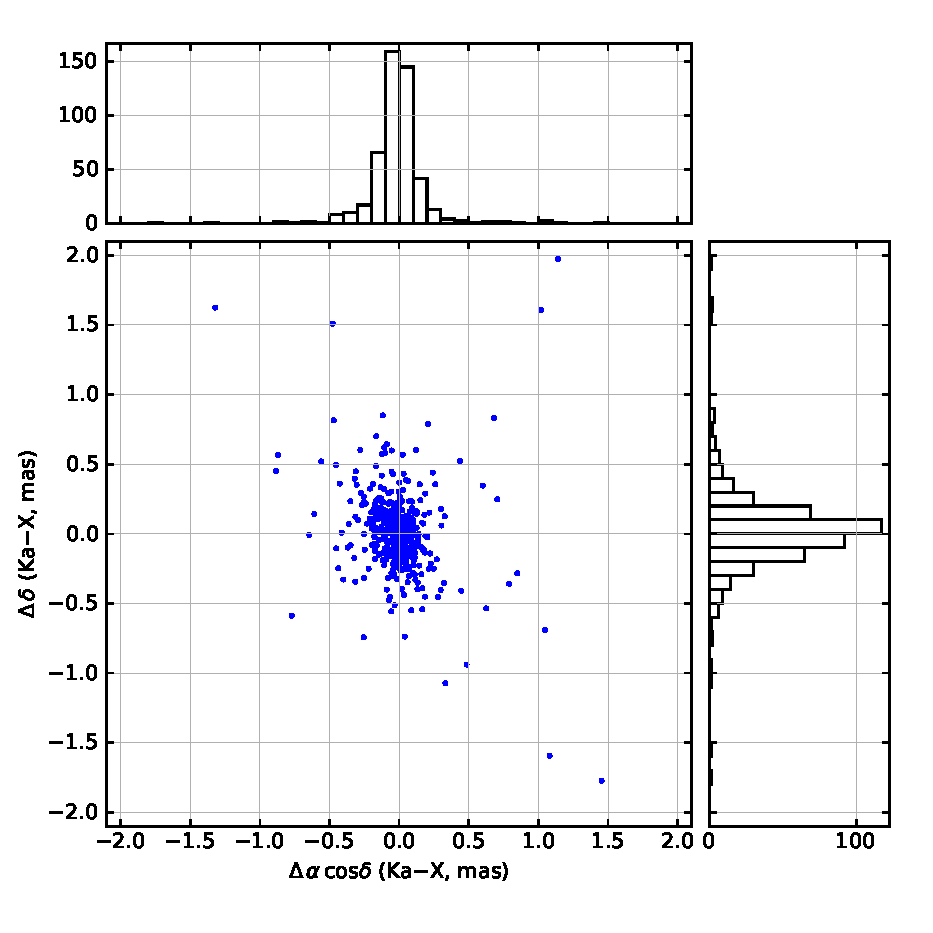
\includegraphics[width=60mm]{figs/xka-sx-scatter}
        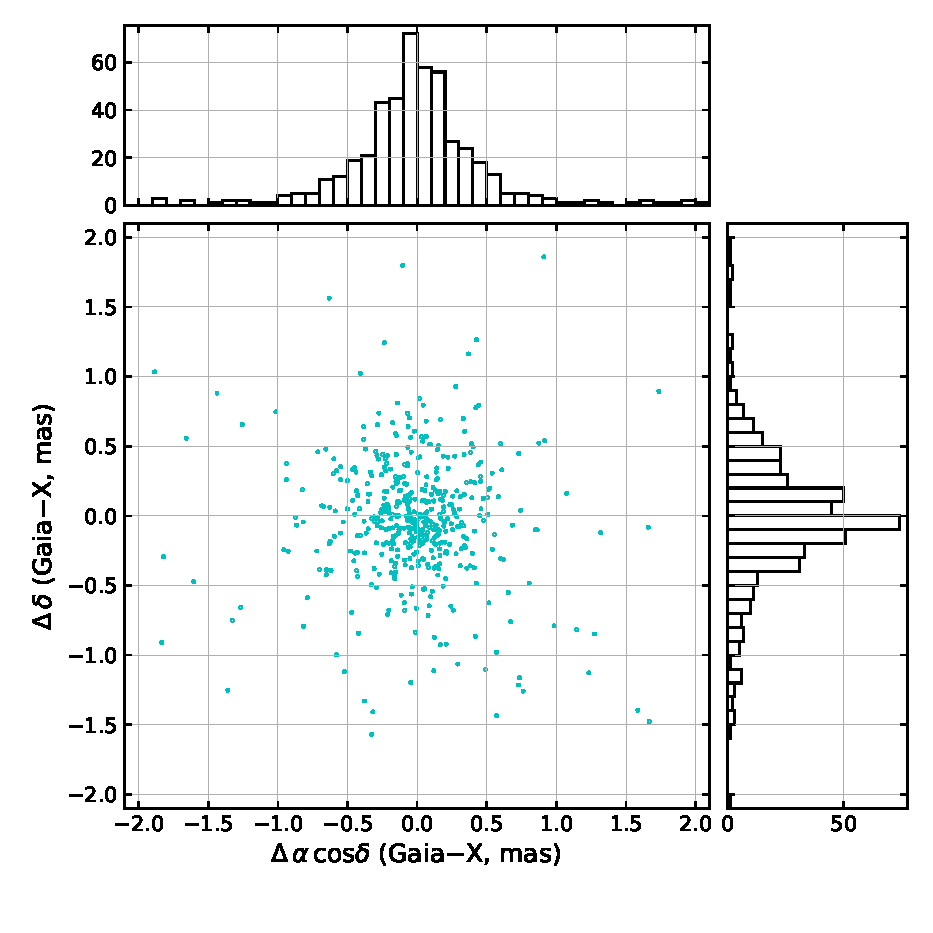
\includegraphics[width=60mm]{figs/gaia-sx-scatter}
        \caption[]{\label{fig:pos-offset-scatter}
            Position offset scatter and distribution of their component in the right ascension and declination for 488 sources of  (Top) $K$-band, (Middle) $Ka$-band, and (Bottom) \textit{Gaia} positions with respective to the $X$-band position after removing the global differences.
        }
    \end{figure}

   Table~\ref{tab:vsh01}-\ref{tab:vsh02} report the VSH parameters of the first and second degree, respectively.
   The transformation parameters between $K$-band and $X$-band position are less than $30\,\mathrm{\mu as}$ except $D_2$ and $E_{21}^I$.
   Similar results could be found in between $Ka$-band and $X$-band; however, significant terms, $D_3$, $E_{20}$, and $M_{20}$ exceeding 0.3~mas are also reported, which would cause a declination bias on the same level.
   %This result justifies the necessity of removing the global difference and aligning the celestial frames at other wavelengths to the $X$-band frame before analyzing of position offsets.
   Most of the transformation parameters between \textit{Gaia} and $X$-band ranges from $30\,\mathrm{\mu as}$ to $50\,\mathrm{\mu as}$.

   Figure~\ref{fig:pos-offset-scatter} presents the position offset scatters of $K$-band, $Ka$-band, and \textit{Gaia} positions relative to the $X$-band position, as well as distributions of their right ascension and declination components for 488 common sources.
   The agreement between $K$-band and $X$-band positions is around 0.1~mas on the right ascension;
   the declination scatter is slightly larger, making the scatter cloud elongating along the declination axis.
   This phenomenon is more pronounced between $Ka$-band and $X$-band.
   The distribution of offset between \textit{Gaia} and $X$-band positions, with a nearly circle-like shape, is flatter than the $K$- and $Ka$-band, showing similar agreements of 0.3--0.5~mas on the right ascension and declination.
   No bias larger than 0.1~mas in neither right ascension nor declination could be observed for all three position offsets.
   As a result, we freed studies of multi-wavelength positions carried out in the next sections from large-scale differences. %due to deformations and alignment issues.

%
%______________________________________________________________

\subsection{Distribution of radio-to-optical offsets}    \label{subsec:r2o-dist}

%__________________________________________________  {fig:rho-hist}
    \begin{figure}[hbtp]
        \centering
        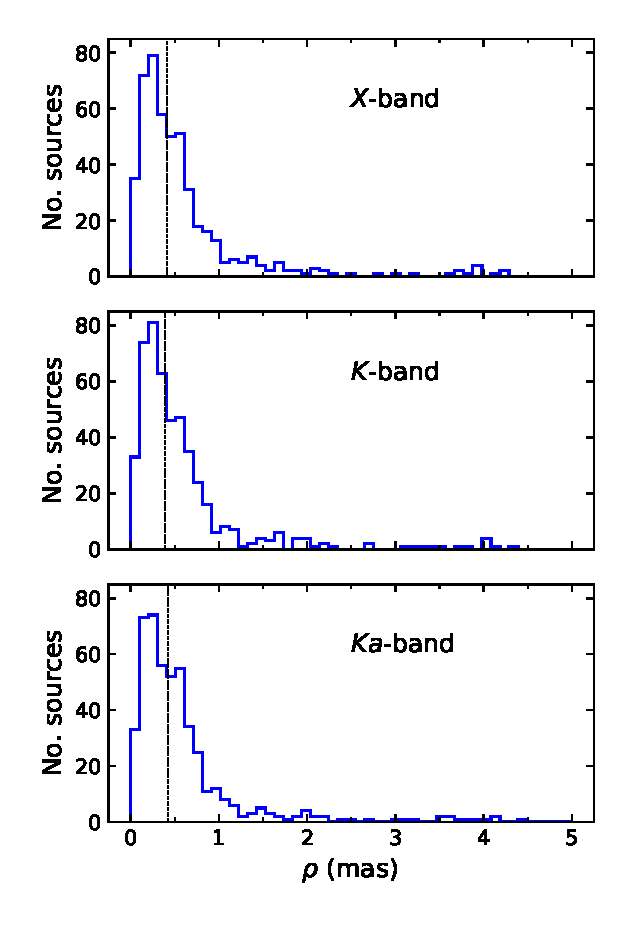
\includegraphics[width=0.45\columnwidth]{figs/rho-hist}
        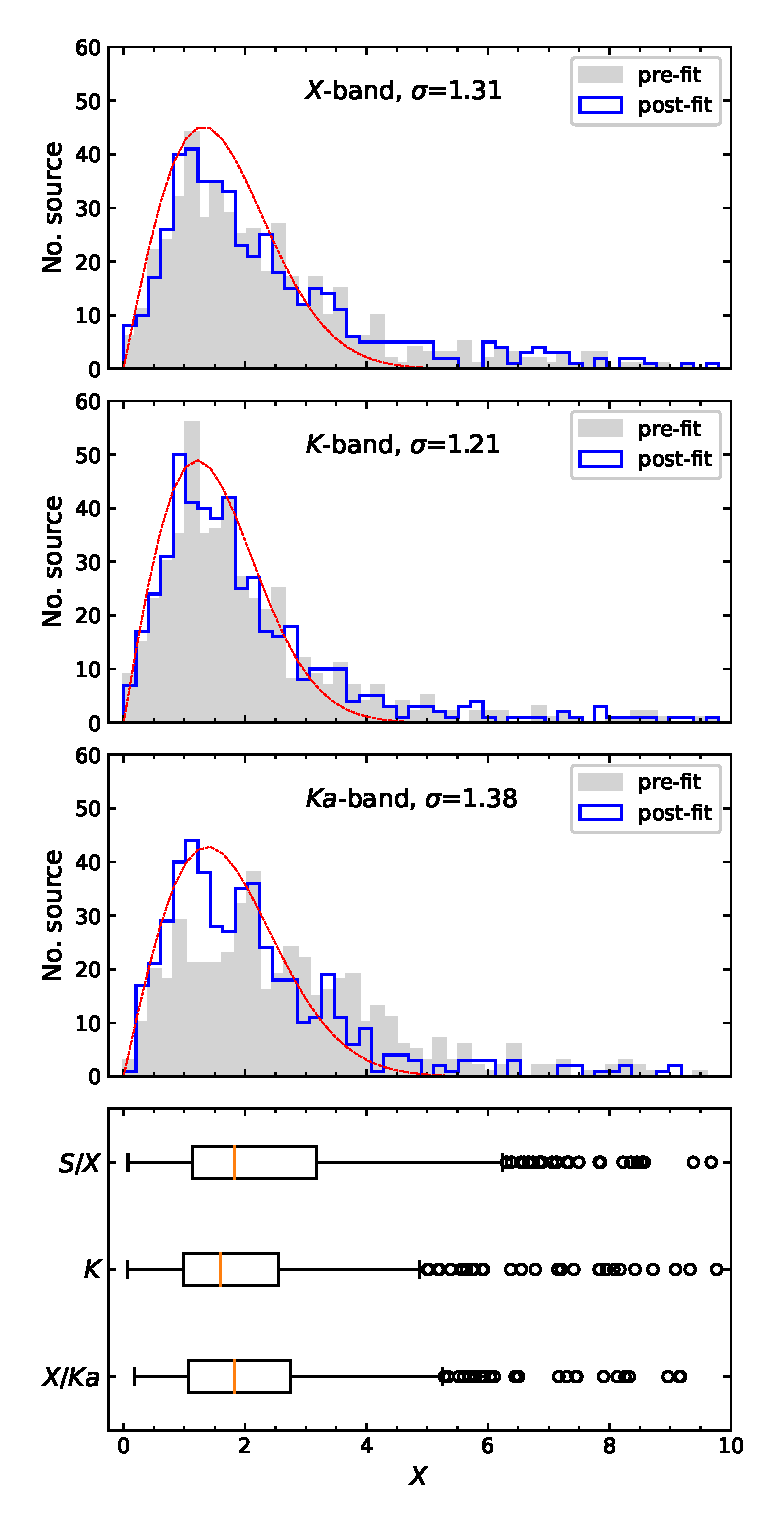
\includegraphics[width=0.45\columnwidth]{figs/X-hist}
        \caption[]{\label{fig:rho-hist}
            Distribution of radio-to-optical offset $\rho$ and normalized separation $X$ at $X$-, $K$-, and $Ka$-band for 488 sources.
            The red dashed curves represent fitted standard Rayleigh distributions based on sources with $X<X_0$.
            The median value of each distribution is indicated by the dark dashed line.
        }
    \end{figure}

    Figure~\ref{fig:rho-hist} depicts the distributions of radio-to-optical offsets at $X$-, $K$-, and $Ka$-band, yielding similar shapes with median values of 0.41~mas, 0.40~mas, and 0.42~mas, accordingly.
    The 5th and 95th percentiles are: 0.08~mas and 2.06~mas at $X$-band; 0.09~mas and 2.01~mas at $K$-band; and 0.09~mas and 2.16~mas at $Ka$-band.
    Only six sources have a radio-to-optical offset larger than 5~mas at either radio bands.
    We found a second peak at around 0.6~mas at all three bands, which is sharpest at the $X$-band.

    The distributions of normalized separations are slightly different: it is sharper for the $Ka$-band while flatter for the $X$-band.
    There are 16 sources at $X$-band, 6 at $K$-band, and 8 at $Ka$-band with $X~>~10$, which are beyond the axis.
    For ideal cases, $X$ is supposed to follow a Rayleigh distribution of unit standard deviation, then the median value of $X$ would 1.18.
    For a sample of $N$ souces, the number of sources with $X>X_0$ is expected to be less than one when $X_0=\sqrt{2\log{N}}$.
    For our sample ($N=488$), the upper limit $X_0$ is 3.52.
    Medians of normalized separations are 1.89, 1.69, and 1.77 for $X$-, $K$-, and $Ka$-band, respectively, all greater than the predicted median value of ideal cases.
    We fitted the normalized separation distributions to the Rayleigh curve with an unknown standard deviation $\sigma$.
    The fitting returns the estimation of $\sigma$ to be 4.01 for $X$-band, 3.16 for $K$-band, and 3.22 for $Ka$-band.
    % If we made a cut-off of 5 on the normalized separation, $\sigma$ would be reduced to 1.57 for $X$-band, 1.39 for $K$-band, and 1.51 for $Ka$-band.
    The distribution of $X$ would become much closer to the unit-standard-deviation Rayleigh shape ($\sigma \simeq 1.3$) if restricting sources to those with $X<X_0$.
    This upper limit would rule out sources with statistically significant radio-to-optical offsets as outliers, whose number is 99 for $X$-band, 64 for $K$-band, and 66 for $K$-band, respectively.

    We further compared three radio-to-optical offsets of individual source. %, as presented in Fig~\ref{fig:rho-vs-si}.
    Except for few cases, the radio-to-optical offsets determined from $X$-, $K$-, and $Ka$-band generally are approximately equal.
    No statistically obvious evidence shows that the radio-to-optical offset decreases at high frequency.
    Further examinations report that the absolute difference among three radio-to-optical offsets for 95\% sources is less than 0.54~mas, which could be considered as a upper limit of the deviation among three radio-to-optical offsets for our sample.
    We observed similar results for normalized separations, regardless the normalized separation at $X$-band is slightly larger than other two bands.

%    We listed four groups of interest as listed below and discussed them in Sect.~\ref{subsec:cause-of-VG}.
    %
%    \begin{itemize}
%        \item[A] 44 sources with radio-to-radio offset < 0.54~mas, radio-to-optical offsets > 1~mas.
%        \item[B] three sources with $X$-to-\textit{Gaia} offset > 1~mas, $K$-to-\textit{Gaia} and $Ka$-\textit{Gaia} offset < 0.54~mas.
%        They are 0629--418, 1129--580, and 2134+004.
%        \item[C] 2 sources with $Ka$-to-\textit{Gaia} offset > 1~mas, $X$-to-\textit{Gaia} and $K$-to-\textit{Gaia} offset < 0.54~mas.
%        They are 1315--058, 1345+289, and 2256--084 .
%        \item[D] 2 sources with $K$-to-\textit{Gaia} offset > 1~mas, $X$-to-\textit{Gaia} and $Ka$-to-\textit{Gaia} offset < 0.54~mas.
%        They are 2227--399 and 1611-710.
%    \end{itemize}

%

%
%__________________________________________________
%
%For example, 2008--159 has an angular separation of $\sim\mathrm{0.2~mas}$ between $X$-band and \textit{Gaia}, $\sim\mathrm{0.1~mas}$ between $Ka$-band and \textit{Gaia} but a few micro-arcseconds for between $K$-band and \textit{Gaia}.
%It suggests that VLBI at $X$-band and $Ka$-band measures the same or close emission center while $K$-band VLBI and \textit{Gaia} measures another one.
%Similar cases could be found, such as 0827+243 with $\rho~(\rm $K$-Gaia) \simeq~\rho~(\rm $Ka$-Gaia)~\simeq~0.01~{\rm mas}$ but $\rho~(\rm $X$-Gaia) \simeq~0.1~{\rm mas}$,
%and 1315--058 with $\rho\,(\rm $K$-Gaia)\,\simeq~\rho~(\rm $X$-Gaia)~\simeq~0.3~{\rm mas}$ but $\rho~(\rm $Ka$-Gaia) \simeq~13.6~{\rm mas}$.



%__________________________________________________

\subsection{Correlation between radio-to-optical offsets and source properties}    \label{subsec:r2o-corr}
%
    Figure~\ref{fig:rho-g-mag} demonstrates a correlation between the radio-to-optical offsets and \textit{Gaia} $G$ magnitude: the radio-to-optical offsets increase towards the faint end for all three radio bands.
    This correlation could be still seen if we included all the common sources between each ICRF catalog and \textit{Gaia}-CRF2 subsets, for instance, the 2820 sources between the ICRF3 $X$-band catalog and \textit{Gaia}-CRF2.
    We also plotted the normalized separation against the $G$ magnitude in the Fig.~\ref{fig:rho-g-mag} and found a slightly decreasing trend for $X$-band and flat trends for $K$- and $Ka$-band at $17\,<\,G\,<\,20$.
    The Spearman correlation coefficient between the radio-to-optical offset $\rho$ and the $G$ magnitude is around 0.5 with
    a high confidence (the $p$-value $<5 \times 10^{-21}$), while the correlation decreases to $-0.2$ when considering the normalized distances.

    We found 142 matches with the structure index information available.
    For most sources, the structure index falls in the range of 2 to 3.5.
    The radio structure index of 322 sources is color-coded in the Fig.~\ref{fig:rho-vs-si}, where we could not detect a obvious correlation. % between the radio-to-optical offsets.

    The redshift measurement are given for 443 sources.
    We did not detect any dependency of neither radio-to-optical angular separation (Fig.~\ref{fig:rho-z}) nor normalized separation (not plotted for brevity) on the redshift.

    In our sample of 488 common sources, 199 sources associated with the morphological index at the filter $B$, 396 at the filter $R$, and 340 at the filter $I$.
    All three morphological indices larger than one were found for 9 sources at the filter $B$, 16 sources at the filter $R$, and 25 sources at the filter $IR$, corresponding to about 5\%, 4\% and 7\% of the subset with these morphological indices available, respectively.
    Figures~\ref{fig:rho-IR} demonstrates a smooth dependency of the radio-to-optical distance on the three morphological index of $R$-filter.
    The morphological index of filter $B$ and $IR$ present similar results to those of filter $R$ and thus are not plotted here.

%%
%__________________________________________________{fig:rho-g-mag}

    \begin{figure*}[hbtp]
        \centering
        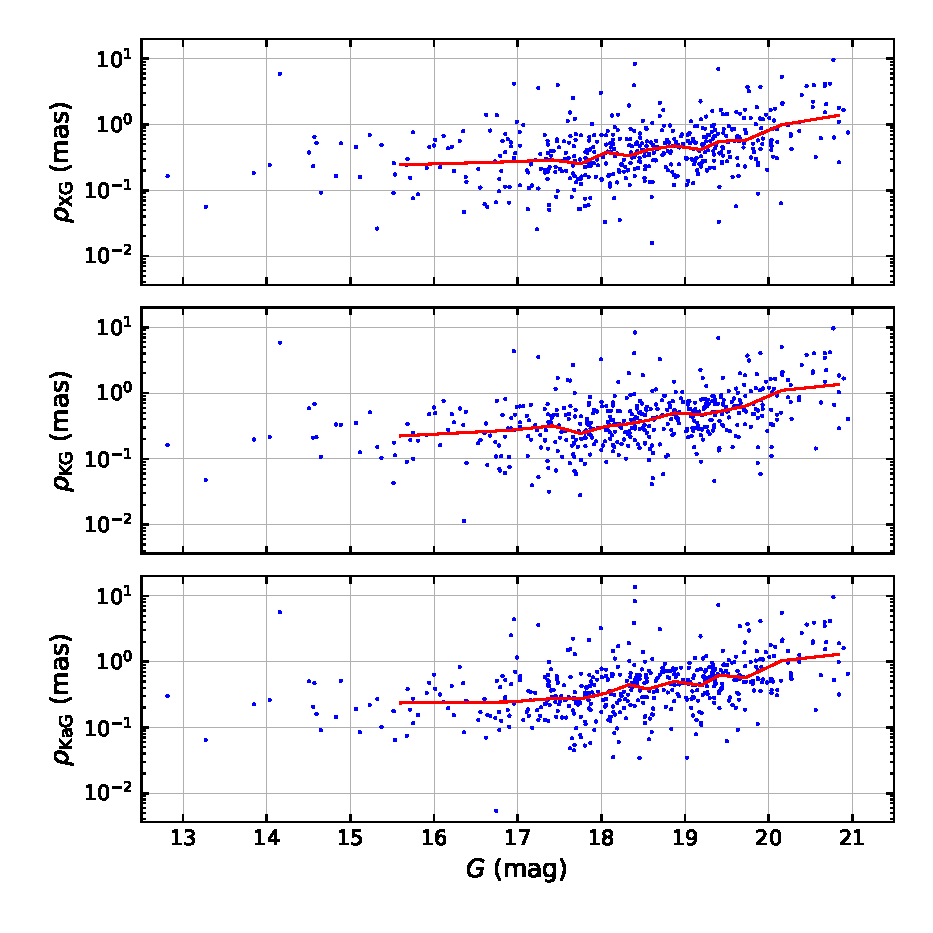
\includegraphics[width=0.6\columnwidth]{figs/rho-g-mag}
        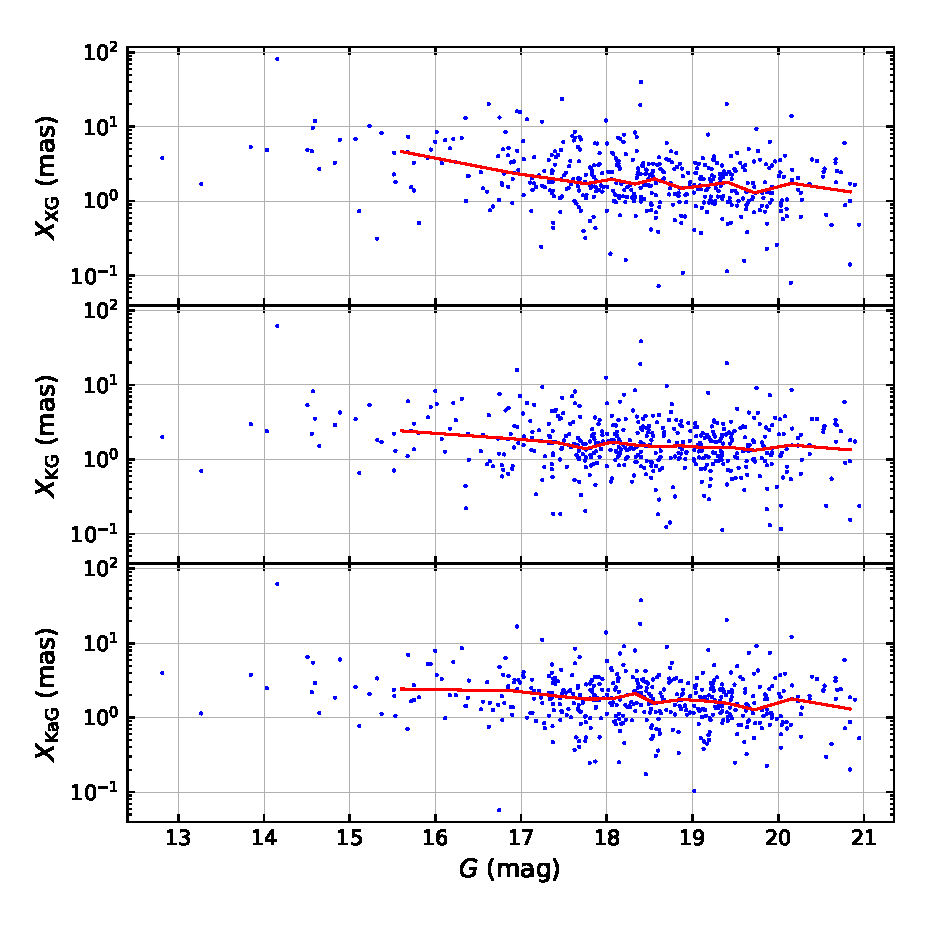
\includegraphics[width=0.6\columnwidth]{figs/X-g-mag}
        \caption[]{\label{fig:rho-g-mag}
            Radio-to-optical offset $\rho$ and normalized separation $X$ at $X$-, $K$-, and $Ka$-band as a function of \textit{Gaia} $G$ magnitude for 488 sources.
            The red dashed line indicates the median values in subsets binned by every 40 sources.
        }
    \end{figure*}

%%
%__________________________________________________{fig:rho-vs-si}
    \begin{figure*}[hbtp]
        \centering
        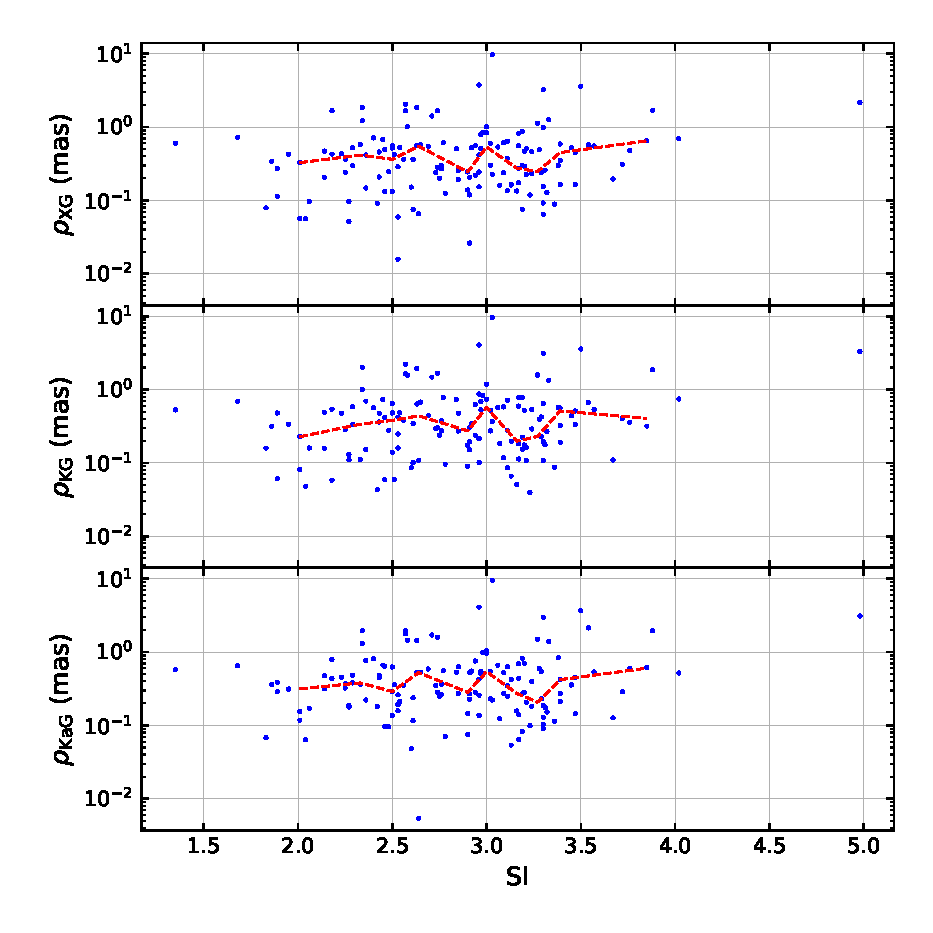
\includegraphics[width=0.6\columnwidth]{figs/rho-si}
        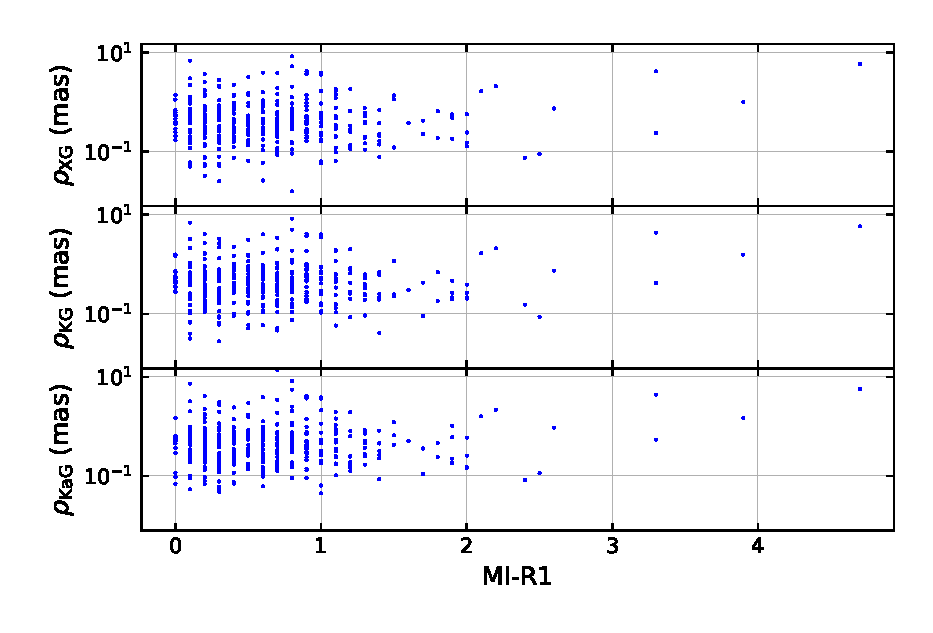
\includegraphics[width=0.6\columnwidth]{figs/rho-I1R}
        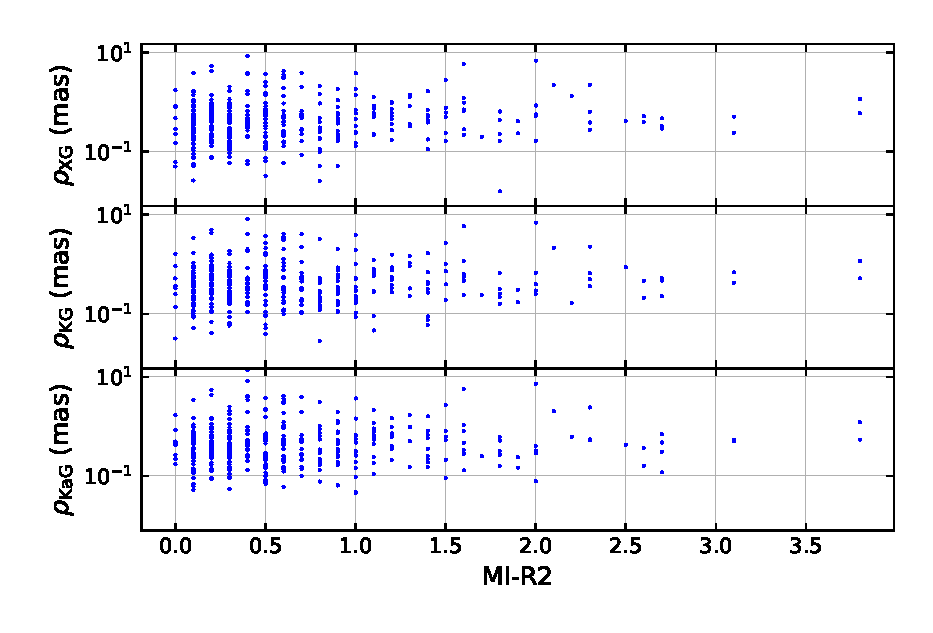
\includegraphics[width=0.6\columnwidth]{figs/rho-I2R}
        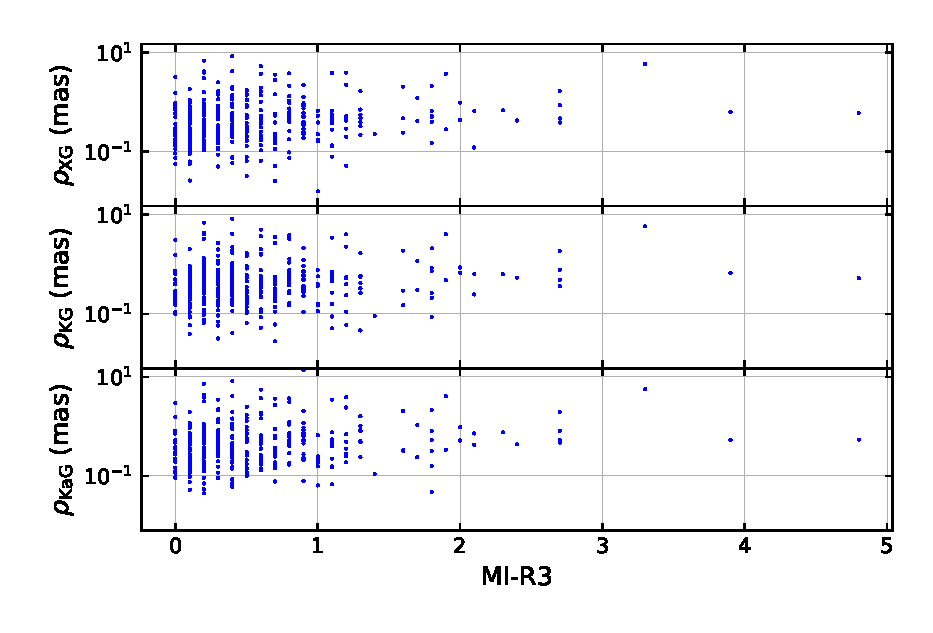
\includegraphics[width=0.6\columnwidth]{figs/rho-I3R}
%        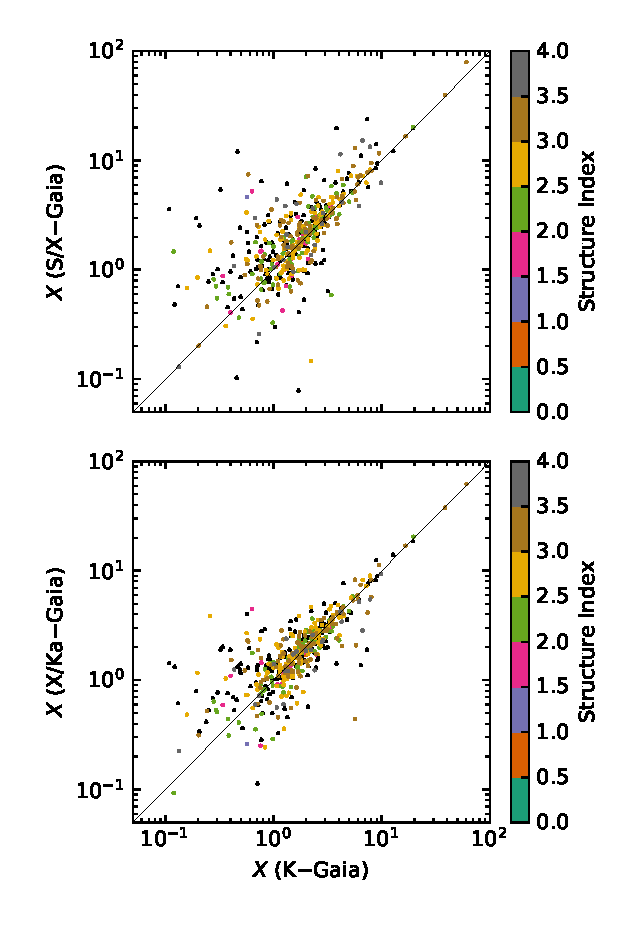
\includegraphics[width=80mm]{figs/X-com-vs-si}
        \caption[]{\label{fig:rho-vs-si}
            Radio-to-optical offset $\rho$ at $X$-, $K$-, and $Ka$-band as a function of source structure index for 142 sources.
            The red dashed line indicates the median values in subsets binned by every 20 sources.
        }
    \end{figure*}

%%
%__________________________________________________{fig:rho-z}

    \begin{figure}[hbtp]
        \centering
        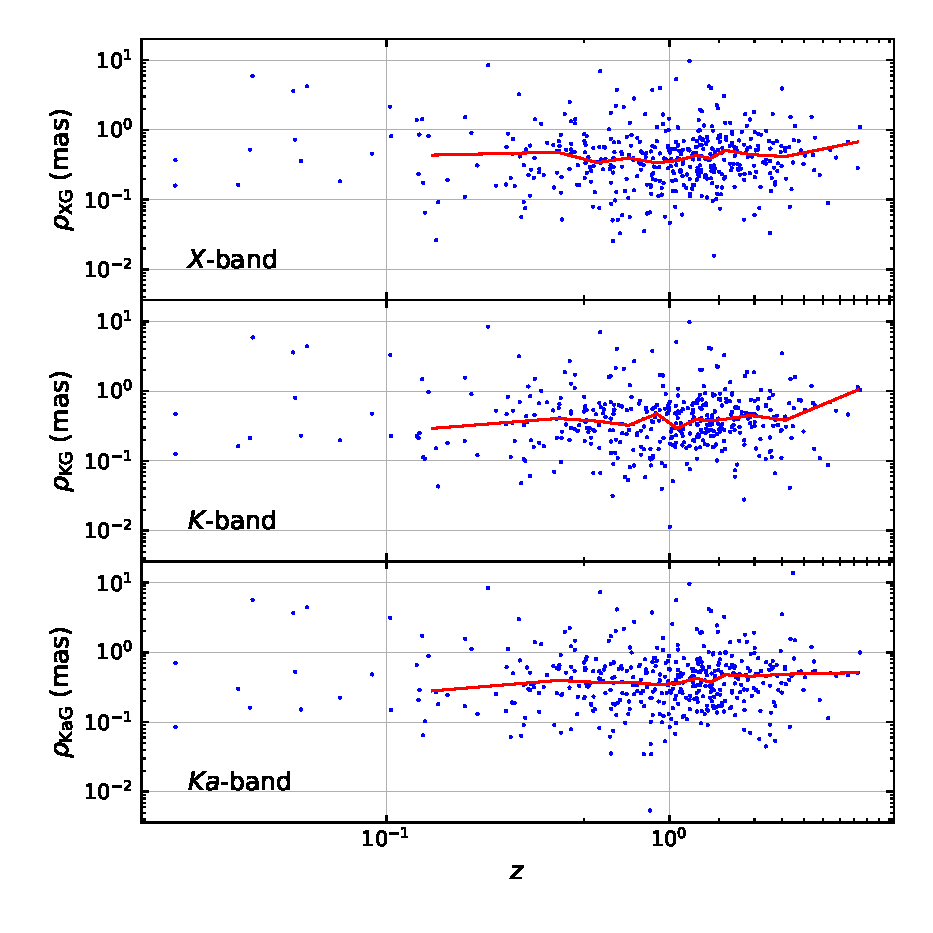
\includegraphics[width=80mm]{figs/rho-z}
        \caption[]{\label{fig:rho-z}
            Radio-to-optical offset $\rho$ at $X$-, $K$-, and $Ka$-band as a function of red-shift $z$ for 443 sources having a red-shift measurements in the LQAC-5 catalog.
            The red dashed line indicates the median values in subsets binned by every 15 sources.
        }
    \end{figure}


%%
%__________________________________________________{fig:rho-IR}
    %
    % \begin{figure}[hbtp]
    %     \centering
    %     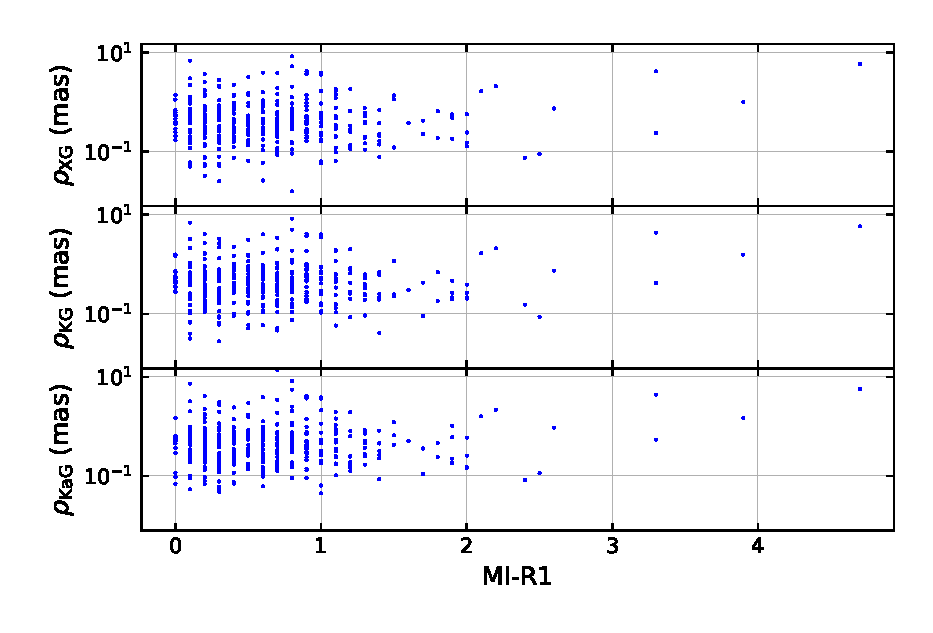
\includegraphics[width=80mm]{figs/rho-I1R}
    %     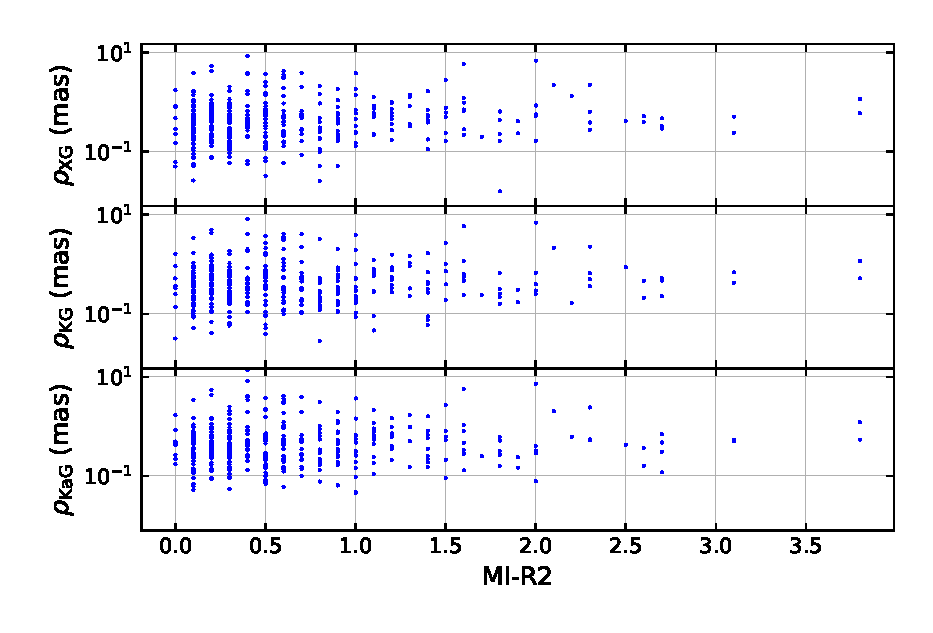
\includegraphics[width=80mm]{figs/rho-I2R}
    %     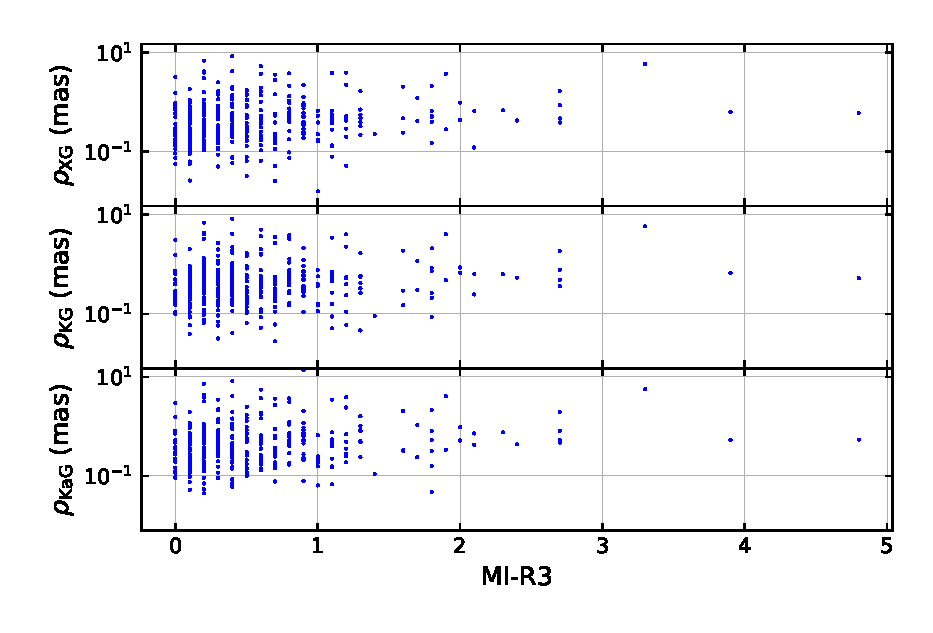
\includegraphics[width=80mm]{figs/rho-I3R}
    %     \caption[]{\label{fig:rho-IR}
    %         Radio-to-optical offset $\rho$ at $X$-, $K$-, and $Ka$-band as a function of morphological index (Top) SHARP, (Middle) SROUND, (Bottom) GROUND at filter R for 396 sources having R-filter morphological indices in the LQAC-5 catalog.
    %
    %     }
    % \end{figure}

%__________________________________________________

\subsection{Aligned multi-wavelength positions}    \label{subsec:pos-align}


    In this section, we used the direction information of the position offset to investigate the relation of multi-wavelength positions for individual source.
    The position angles of $K$-band, $Ka$-band, and \textit{Gaia} positions with referred to the $X$-band position are plotted in Fig.~\ref{fig:pa-hist}.
    Peaks at around $0\,^\circ$, $180\,^\circ$, and $360\,^\circ$ could be observed for $K$- and $Ka$-band positions, while \textit{Gaia} position does not show a similar preference.

    In order to compare the position angles of $K$-band, $Ka$-band, and \textit{Gaia} positions with respective to the $X$-band position,
    we calculated the differences between these position angles and wrapped them into the range of $-180\sim180^\circ$.
    Figure~\ref{fig:pa-diff} depicts the distribution of position angle differences, where one could observe a clear peak around $0^\circ$ above the mean value (red dashed line) while no peak appears at $\pm 180^\circ$.
    If we set a limit on the position angle difference, below which the multi-wavelength positions could be considered as aligned, the number of sources for different cases is summarized in the Table~\ref{tab:no_sou_aligned}.
    Note that only for sources with all (at least two) normalized separations $\rho_{\rm w}>1$ with respective to the $X$-band position, the derived position angle is reliable.
    Taking this condition into consideration reduces the subsets of sources with aligned positions to nearly their half-size.

    We adopted a limit of $30^\circ$ on the absolute PA difference and the condition of $\rho_{\rm w}>1$ for further analysis.
    As a result, we obtained a sample of 47 sources having positions at  four frequencies aligned, among which we found the jet information for 20 sources from \citep{2019ApJ...874...43L}.
    Figure~\ref{fig:jet-pa-com} depicts the distribution of the difference between the jet direction and \textit{Gaia}-to-X offset vector.
    Again, we considered an absolute PA difference limit of $30^\circ$, therefore, six sources have the radio-to-optical offset in the downstream direction while five sources with PA difference yields a radio-to-optical offset in the upstream of the jet.
    We compared the position offset vectors with the VLBA image and found that the positions at four bands are usually located within the compact core (<0.5~mas) except for few cases.
    F%or example, 1157-215 as exemplified in Fig.~\ref{fig:illustration-diagram} shows two-core structure, with $X$-band focusing one component, $Ka$-band and \textit{Gaia} for another one, and $K$-band for intermediate part.

    Table~\ref{tab:aligned-sou} tabulates the position offsets of $K$-band, $Ka$-band, and \textit{Gaia} positions with respective to the $X$-band position for 47 sources whose four-band positions are aligned. %, as well as the jet direction if available.
    Position offsets in the downstream and upstream side of jet are plotted in Figs.~\ref{fig:jet-down} and \ref{fig:up}.

%%
%__________________________________________________{fig:pa-hist}

    \begin{figure}[hbtp]
        \centering
        \includegraphics[width=\columnwidth]{figs/pa-hist}
        \caption[]{\label{fig:pa-hist}
            Distribution of the position angle of offset vector of $K$-band, $Ka$-band, and \textit{Gaia} positions with referred to the $X$-band position for 488 common sources.
            The horizontal red dashed line stands for a uniform distribution.
        }
    \end{figure}

%%
%__________________________________________________{fig:pa-diff}

    \begin{figure}[hbtp]
        \centering
        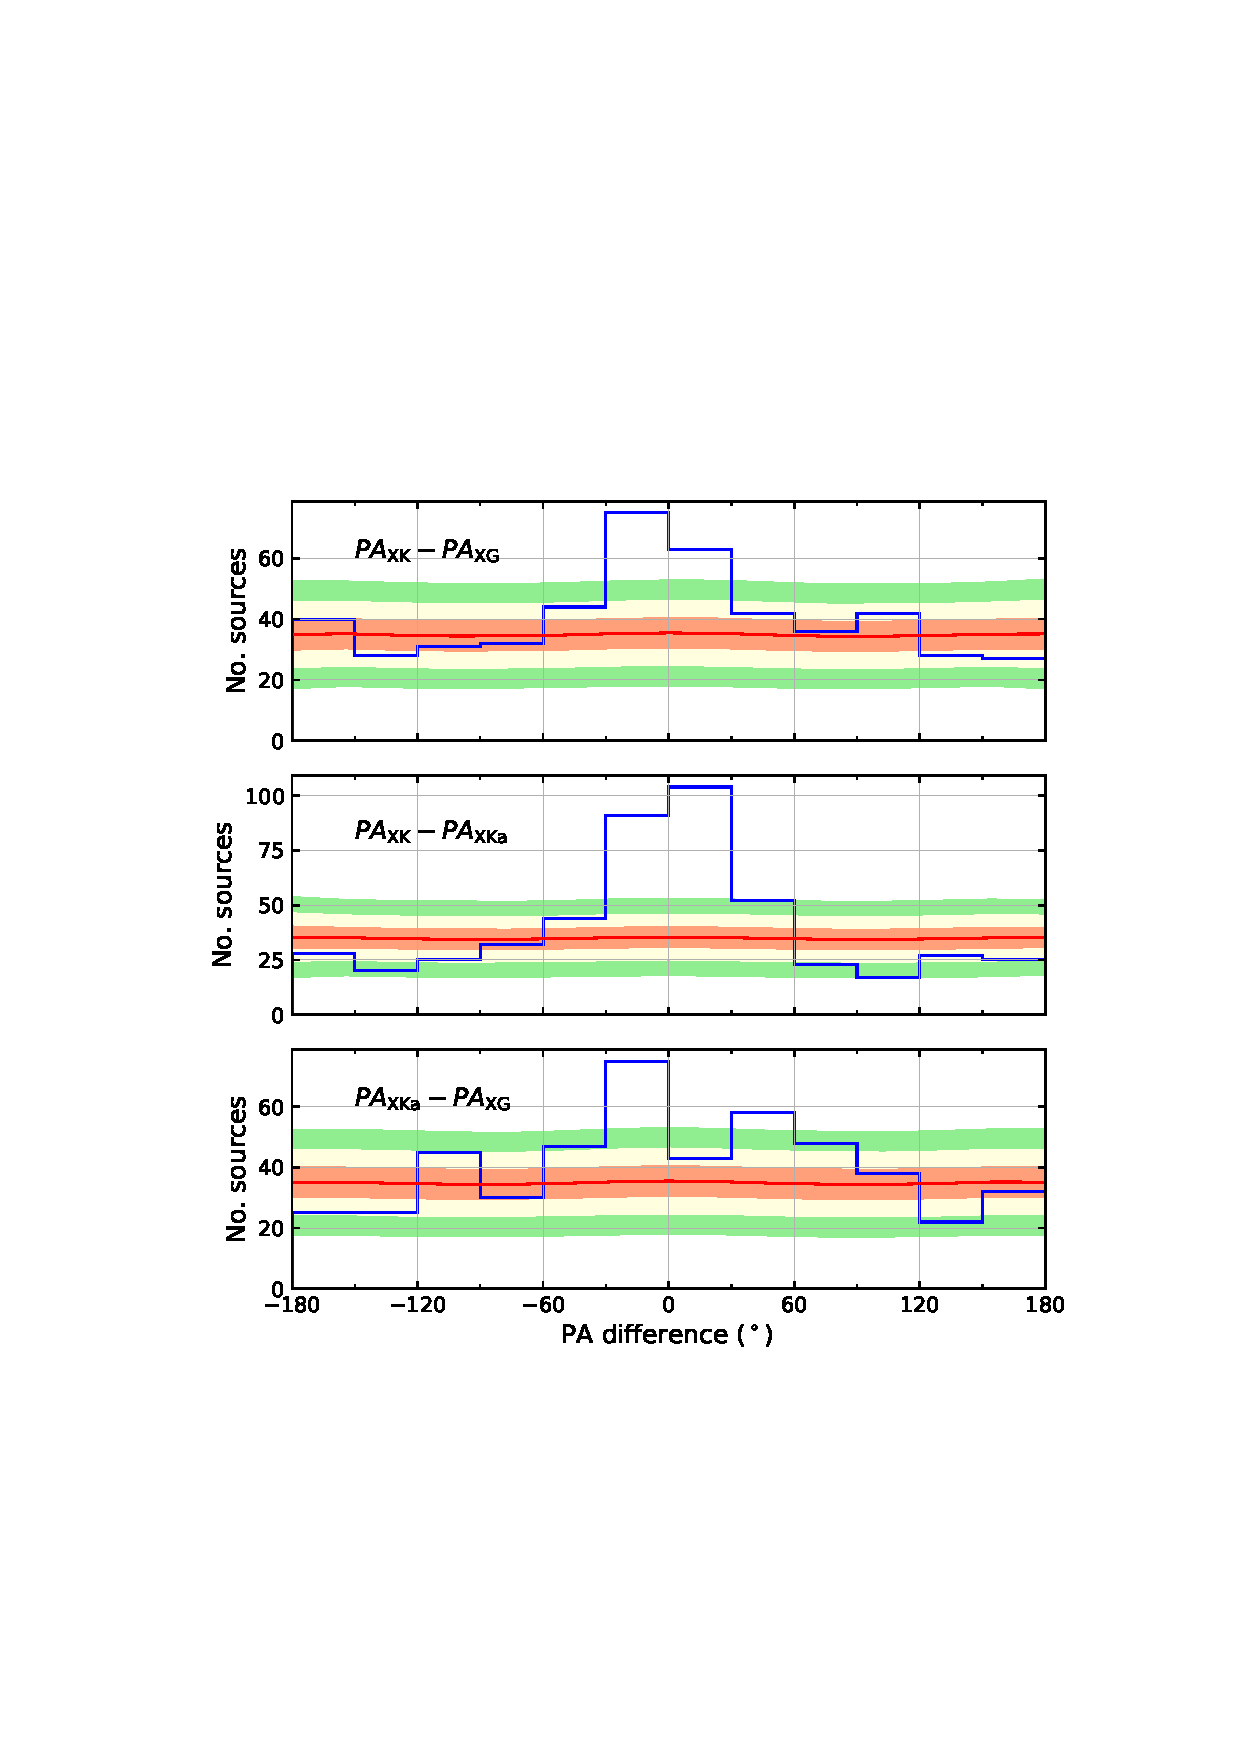
\includegraphics[width=\columnwidth]{figs/pa-diff.png}
        \caption[]{\label{fig:pa-diff}
            Distribution of the position angle difference of offset vector of $K$-band, $Ka$-band, and \textit{Gaia} positions with referred to the $X$-band position for 488 common sources.
%            The horizontal red dashed line stands for a uniform distribution.
            The red curve stands for mean histogram and shading zones represent the confidence intervals of 1-$\sigma$ (standard deviation) to 3-$\sigma$.
        }
    \end{figure}

%%
%__________________________________________________{fig:jet-pa-co}

    \begin{figure}[hbtp]
        \centering
        \includegraphics[width=\columnwidth]{figs/jet-pa-com}
        \caption[]{\label{fig:jet-pa-com}
            Distribution of the position angle difference of $X$-to-\textit{Gaia} position offset vector and jet vector for 20 sources whose four-band positions are almost aligned ($|\Delta PA|~<~30^{\circ}$).
        }
    \end{figure}

%% {fig:illustration-diagram}
%__________________________________________________ {fig:killustration-diagram}
%\begin{figure}[hbtp]
%    \centering
%    \includegraphics[width=70mm]{figs/1157-215}
%    \includegraphics[width=70mm]{figs/1157-215.u.2013_05_05.icn_color.png}
%    \caption[]{\label{fig:illustration-diagram}
%        Top: Position offset vectors of $K$-band, $Ka$-band, and {\it Gaia} (optical) positions with respect to the $X$-band position for source 1157--215.
%        Around the positions is the error ellipse of 1-$\sigma$ at each band.
%        Also shown is the jet direction taken from MOJAVE database whilst the magnitude (length) is arbitrary and thus meaningless.
%        Bottom: Image from MOJAVE database for comparison.
%    }
%\end{figure}
%%
%__________________________________________________{tab:no_sou_aligned}

    \begin{table*}[htbp]
        \centering
        \caption{\label{tab:no_sou_aligned}
            Number of sources with multi-wavelength positions aligned.
        }
        \begin{tabular}{ccccc}
            \hline \noalign{\smallskip}
            &$X$, $K$, $Ka$ &$X$, $K$, \textit{\it Gaia} &$X$, $Ka$, \textit{\it Gaia} &$X$, $K$, $Ka$, \textit{\it Gaia}\\
            \noalign{\smallskip}
            \hline
            \noalign{\smallskip}
            $|\Delta PA|<45^\circ$       &256  &183  &174  &96\\
            $|\Delta PA|<30^\circ$       &195  &138  &118  &55\\
            $|\Delta PA|<15^\circ$       &106  &73   &74   &24\\
            $|\Delta PA|<45^\circ, \rho_{\rm w}>1$  &156  &97   &110  &74\\
            $|\Delta PA|<30^\circ, \rho_{\rm w}>1$  &122  &75   &82   &47\\
            $|\Delta PA|<15^\circ, \rho_{\rm w}>1$  &75   &45   &52   &24\\
            \hline
        \end{tabular}
    \end{table*}

%%
%__________________________________________________{tab:aligned-sou}
    %
    % \begin{table*}
    %     \centering
    %         \caption{\label{tab:aligned-sou}
    %         Sources with positions at four bands aligned within $30~^\circ$.
    %     }
    %     \begin{tabular}{cccccccccccc}
    %     \hline \noalign{\smallskip}
    %         IERS name & $\rho_{\rm X-K}$ & $PA_{\rm X-K}$ & $\rho_{\rm X-Ka}$ & $PA_{\rm X-Ka}$ & $\rho_{\rm X-G}$ & $PA_{\rm X-G}$ & $PA_{\rm jet}$ & SI & SHARP & SROUND & GROUND \\
    %         & $\mathrm{mas}$ & $\mathrm{{}^{\circ}}$ & $\mathrm{mas}$ & $\mathrm{{}^{\circ}}$ & $\mathrm{mas}$ & $\mathrm{{}^{\circ}}$ & $\mathrm{{}^{\circ}}$ &  &  &  &    \\
    %         \hline \noalign{\smallskip}
    %         % Downstream
    %         0552+398 & 0.1 & 334 & 0.1 & 327 & 0.2 & 329 & 358 & 3.1 & 0.1 & 0.3 & 0.2 \\
    %         0859-140 & 0.4 & 196 & 0.3 & 199 & 0.2 & 204 & 178 & - & 0.9 & 0.4 & 0.2 \\
    %         1157-215 & 2.3 & 317 & 3.5 & 318 & 4.0 & 317 & 324 & - & - & - & - \\
    %         1243-072 & 0.0 & 281 & 0.1 & 263 & 0.6 & 256 & 268 & 2.9 & 0.1 & 0.9 & 0.9 \\
    %         1742-078 & 0.4 & 185 & 0.4 & 184 & 1.2 & 182 & 169 & - & - & - & - \\
    %         2134+004 & 1.1 & 120 & 1.3 & 126 & 1.4 & 126 & 96 & - & 0.0 & 0.5 & 0.4 \\
    %         \hline \noalign{\smallskip}
    %         % Upstream
    %         0430+052 & 0.7 & 61 & 0.7 & 68 & 0.5 & 75 & 258 & - & 0.3 & 2.6 & 1.8 \\
    %         0723-008 & 1.6 & 149 & 2.0 & 148 & 1.4 & 148 & 343 & - & 1.5 & 1.0 & 0.6 \\
    %         0743-006 & 0.4 & 214 & 1.1 & 227 & 1.0 & 233 & 42 & 3.3 & 0.6 & 1.6 & 0.1 \\
    %         0850+581 & 0.8 & 322 & 0.5 & 327 & 0.7 & 336 & 153 & - & 0.3 & 0.2 & 0.2 \\
    %         2251+158 & 0.4 & 72 & 0.4 & 81 & 0.5 & 75 & 280 & - & 0.1 & 0.7 & 0.5 \\
    %         \hline \noalign{\smallskip}
    %         % Other
    %         0003+380 & 0.1 & 106 & 0.1 & 133 & 8.4 & 130 & 96 & - & 0.8 & 0.4 & 0.4 \\
    %         0112-017 & 0.6 & 263 & 0.6 & 276 & 0.7 & 276 & 146 & - & 0.2 & 0.1 & 0.3 \\
    %         0122-003 & 0.5 & 330 & 0.8 & 353 & 0.6 & 358 & 276 & - & 1.0 & 1.1 & 0.8 \\
    %         0133+476 & 0.1 & 94 & 0.2 & 98 & 0.2 & 116 & 331 & 2.3 & 0.3 & 1.0 & 1.8 \\
    %         0917+449 & 0.3 & 169 & 0.4 & 156 & 0.3 & 150 & 197 & - & 1.0 & 1.0 & 0.2 \\
    %         0953+254 & 0.3 & 29 & 0.3 & 50 & 0.8 & 49 & 264 & 3.0 & 0.4 & 0.1 & 0.5 \\
    %         1038+064 & 0.2 & 345 & 0.1 & 347 & 0.4 & 350 & 137 & - & - & - & - \\
    %         1751+288 & 0.1 & 156 & 0.2 & 149 & 0.3 & 141 & 16 & 2.0 & 0.3 & 2.7 & 0.5 \\
    %         2234+282 & 0.4 & 227 & 0.3 & 204 & 0.5 & 219 & 151 & - & 0.2 & 0.6 & 0.6 \\
    %         \hline \noalign{\smallskip}
    %     \end{tabular}
    %     \tablefoot{
    %     Sources are divided into three groups:
    %     (Top) \textit{Gaia} positions in the downstream of jet with respect to the $X$-band positions;
    %     (Middle) \textit{Gaia} positions in the upstream of jet;
    %     (Bottom) others.
    %     The first column gives the source name of IERS designation .
    %     The columns 2-3, 4-5, 6-7 present the angular separation $\rho$ and position angle of $K$-X, $Ka$-X, and \textit{Gaia}-X offset.
    %     The eighth column contains the jet direction collected from the Table~4 in \citet{2019ApJ...874...43L}, followed by the source structure index provided by BVID database.
    %     The last three columns list the morphological index, namely, SHARP, SROUND, and GROUND, at R filter taken from the LQAC-5 catalog.
    %     The ``-'' symbol means that the corresponding information is not available.
    % }
    % \end{table*}

%__________________________________________________

\subsection{Validation from the Monte-Carlo simulation} \label{subsec:simulation}

%__________________________________________________{fig:sim-comp}

%    \begin{figure*}[hbtp]
%        \centering
%        \includegraphics[width=80mm]{figs/sim-rho-vs}
%        \includegraphics[width=80mm]{figs/sim-pa-vs}
%        \caption[]{\label{fig:sim-comp}
%            Simulated distances (left) and position angles (right) of $K$-to-$X$, $Ka$-to-$X$, and \textit{Gaia}-to-$X$ vectors versus those calculated from the given positions in catalogs (original).
%        }
%    \end{figure*}

%__________________________________________________{fig:sim-pa-diff}

%    \begin{figure}[hbtp]
%        \centering
%        \includegraphics[width=80mm]{figs/sim-pa-offset.png}
%        \caption[]{\label{fig:sim-pa-diff}
%            Distribution of the simulated position angle difference of offset vector of $K$-band, $Ka$-band, and \textit{Gaia} positions with referred to the $X$-band position for 488 common sources.
%            The red curve stands for mean histogram and shading zones represent the confidence intervals of 1-$\sigma$ (standard deviation) to 3-$\sigma$.
%        }
%    \end{figure}

     We wanted to test if the peak around zero in Fig.~\ref{fig:pa-diff} was caused by chance.
     We performed a Monte-Carlo simulation by creating 1000 random permutations of the positions in each catalogs and calculating the orientation (PA) of their position offset vectors.
     Then we computed the mean histogram and its standard deviation.
     This procedure was done between $K$- and $X$-band positions, between $Ka$- and $X$-band positions, and between \textit{Gaia} and $X$-band positions, separately.
     Figure~\ref{fig:pa-diff} presents the results of simulation.
     The peak of the ``true'' data histogram is peaking well above three times the standard deviation, making the alignment very significant.

%     I used monte-carlo testing of the null hypothesis by creating 1000 random permutations of the positions in each catalogs. Then I  (Attached plot: the grey levels are 1, 2, and 3 standard deviations around the mean; )

%     In order to check the influence of asymmetry in VLBI position formal uncertainty on the determination of position angle, we also made a Monte-Carlo simulation with considering perturbations following the error ellipse on the ``true'' position at each wavelength.
%     For details of the simulation, please refer to Appendix~\ref{app:sim}.
%     We created 1000 positions for each sources at each wavelength and calculated the distances and position angles of $K$-, $Ka$-band, and \textit{Gaia} positions with referred to the $X$-band one.
%     For individual source, we adopted the peak value of the simulated sample (10000 points) as the estimated value for distance and position angle.
%     Then these estimated values were compared with those from positions given in the catalogs (original value), as presented in Fig.~\ref{fig:sim-comp}.
%     We found that the simulated positional distances agree well with the calculated ones, except a offset floor of $\sim$0.1~mas.
%     The positional uncertainties for these sources with
%     It suggests an agreement budget of 0.1~mas level for source positions at different wavelengths, even though a small offset would be obtained from the original catalog.
%     As for the position angles, the simulated values are consistent with the original one.
%     A small sinusoidal-like pattern is seen but not dominant (amplitude < $10^
%     {\circ}$), whose cause is not clearly understood yet.
%     We also computed the mean histogram and its standard deviation of the PA differences between $K$-to-$X$, $Ka$-to-$X$, and \textit{Gaia}-to-$X$ vectors.
%     From Fig.~\ref{fig:sim-pa-diff}, the excesses around $0^{\circ}$ are still pronounced, above the 3-sigma level.

%__________________________________________________

\section{Discussion} \label{subsec:discussion}
%
%__________________________________________________

\subsection{Cause of radio-to-optical distance} \label{subsec:cause-of-VG}
%
    \citet{2017MNRAS.471.3775P} summarize several causes for non-coincidence of the emission centers measured by the VLBI and \textit{Gaia}.
    They includes:\\
    (1) large uncertainties in the \textit{Gaia} or/and VLBI positions;\\
    (2) optical structure (jet) at mas-scale; \\
    (3) optical position shift due to luminous host galaxy or asymmetry structure;\\
    (4) radio source structure and core-shift effect;\\
    (5) gravitational lensing and dual AGNs.\\
    We checked these items based on our results except the second one that has been studied deeply in \citet{2017A&A...598L...1K,2017MNRAS.467L..71P,2017MNRAS.471.3775P,2019MNRAS.482.3023P,2019ApJ...871..143P,2020MNRAS.493L..54K}. %, and the last one which happens for few cases.

    The \textit{Gaia} astrometric precision gets worse as one moves to the faint end, and this holds true for quasar positions \citep{2016A&A...595A...5M,2018A&A...616A..14G}, while VLBI formal error does not yield such a dependency.
    We observed that the radio-to-optical offsets increase slightly with the $G$-magnitude in the range of $17<G<21$, as presented in Fig.~\ref{fig:rho-g-mag}.
    It justifies the criterion of being optically bright for selecting suitable optical-to-radio frame-tie sources in \citet{2008A&A...490..403B}.
    However, the angular separations between VLBI and \textit{Gaia} positions are flat or even decrease at $X$-band.
    These results suggest that the large offsets at the fainter end are accounted by the \textit{Gaia} formal error, making them less significant.
    \citet{2020A&A...634A..28L} also suggest that the global accuracy of the \textit{Gaia}-CRF2 does not degrade with increasing the limiting magnitude of the sample.
    Hence, the objects for future link between \textit{Gaia}-CRF and ICRF may not have to be optically bright.

    The radio source structure seen at low frequencies might shift the radio position at $X$-band while the $K$- and $Ka$-band positions are less affected.
    If the strong source structure exists in the most radio sources, the radio-to-optical distance would significantly decrease at higher frequencies.
    We did not observe such a tendency;
    instead, the $X$-, $K$-, and $Ka$-band positions show offsets at the similar level to the \textit{Gaia} position (See Fig.~\ref{fig:rho-vs-si}).
    The structure index for sources with a radio-to-optical distance larger than 1~mas mainly exceeds 2.5, suggesting that large radio-to-optical distance is usually associated with a large structure index.
    It justifies again the selection criterion that frame-tie sources should have a small value of structure index in \citet{2008A&A...490..403B}.
    %But one should note that for these sources, the extend source structure at $X$-band does not seem to diminish at $K$- and $Ka$-band.

    \citet{2017ApJ...835L..30M} find that the radio-to-optical distance becomes significant at $z<0.5$.
    They infer that the shift of \textit{Gaia} position due to the extend optical structure effect explains partly the significant radio-to-optical distance, and this effect would become smaller as moving far away.
    The radio-to-optical distance does not correlate with the redshift as seen from our sample (Fig.~\ref{fig:rho-z}).
    At the interval of $z<0.5$, the number of sources becomes sparse, preventing us from drawing any conclusion within this range.

    Since there are only few cases with larger morphological indices than 1, the influence of the host galaxy on the \textit{Gaia} position, if exist, is not significant for the bulk of our sample.
    %The radio-to-optical offset does not show obvious correlations with the morphological indices as expected.
    Since these indices were determined from the optical imaging with a resolution of arc-seconds or worse, we could not use them to probe the mas-scale optical jet.
    Morphological indices based on high-resolution images might be useful to infer the existence of the mas-scale optical jet found by \citet{2017MNRAS.467L..71P}.

    The radio-to-optical offsets at different bands are roughly at same level, with a deviation of <~0.54~mas for most sources.
    For individual source, however, radio-to-optical offsets might be significantly inconsistently.
    For instance, for 1315--058 the radio-to-radio offsets at $X$- and $K$-band is around 0.3~mas, but at $Ka$-band it is as large as 13.60~mas.
    A possible explanation could be that \textit{Gaia} measures position of the same radio component as the $K$- and $X$-band do, while the $Ka$-band measures another one.

    %\textcolor{red}{We picked out sources according to their radio-to-radio and radio-to-optical offsets in Sect.~\ref{subsec:r2o-dist}.
%    For sources in the group A, radio cores all locate far from the optical core, indicating that the radio-optical offset is more likely related to the shift of optical position.
%    We compared our list with those in \citet[][their Table~1]{2017ApJ...835L..30M}, and found that 4 sources were labeled as ``galaxy'' and 2 sources were recognized as double component therein.
%    The former case means that the optical centroid measured by \textit{Gaia} is perturbed by the luminous host galaxy or asymmetry dust structures.
%    As for two sources in the gourp B, the
%    Similar explanations also works for the group C and D.}



%__________________________________________________

\subsection{Frequency-position relation} \label{subsec:freq-pos}

    The preferred angle in Fig.~\ref{fig:pa-diff} is zero while no peak shows up at 180 degree, indicating that the $K$-band, $Ka$-band, and \textit{Gaia} positions are on the same side of the $X$-band position.
    This result differs from that expected from the north-south systematics in $K$- and $Ka$-band frame with respective to the $X$-band and \textit{Gaia} frames as shown in Fig.~\ref{fig:pa-hist}.
    The simulation results also support that the peak at $0^{\circ}$ is genuine, not be biased by the asymmetry position error of individual source.

    We found 47 sources, about 10\% of the sample, showing roughly aligned positions within $30~^\circ$ at four frequencies.
    Among these sources, 11 out of 20 sources ($>50\%$) with available jet direction information have the radio-to-optical vector parallel to the jet vector.
    If this result holds true for a large sample, it might serve as an astrometric method of determining the jet direction.

    From a simple core-jet model, the optical emission is at the base of the jet while radio cores are shifted along the jet.
    Therefore, we could predict that the dominant scheme of the source positions is, staring from jet upstream, \textit{Gaia} coming first (closest to the black hole), followed by the $Ka$-, $K$-, and $X$-band position.
    For five sources whose four position aligned within $30~^\circ$ with \textit{Gaia} position in the jet upstream, their multi-wavelength positions do not follow this scheme.
    We also note that on the full sample, most of the sources are not aligned.
    As a result, the multi-wavelength comparison suggests that the gross population of the radio sources is not following a simple core-jet model but possibly more complex systems like multi-black holes or various components emitting in different wavelengths.

%\textcolor{red}{The core-shift effect produces a frequency-dependent shift along the jet between the radio core and the jet base.
%It suggests that the multi-wavelength quasar positions would follow a sequence of \textit{Gaia}--$Ka$--$K$--$X$ towards to the jet downstream.
%However, only few sources follows such a position sequence, for example, 1157--215 as shown in the upper panel of Fig.~\ref{fig:illustration-diagram}.
%We assumed that the \textit{Gaia} position to be the jet base and fitted the three radio positions of 1157--215 to the core-shift relation $r(\nu) = r_0\cdot\nu^{-k}$.
%The fitting shows the spectral index to be nearly $-1$, which differs from the result of $k=1$ as predicted in \citet{2009A&A...505L...1P,2008A&A...483..759K}.
%However, our simple derivation of the spectral index $k$ is far from robust and reliable.
%But it worths revisiting the core-shift effect when the new VLBI solutions or \textit{Gaia} data are published.}

%%


%__________________________________________________

\subsection{Influence from the large-scale difference} \label{subsec:sys-effect}

    Our previous work reports that the global differences amongst ICRF3 and \textit{Gaia}-CRF2 catalogs would bias the radio-to-optical offset studies \citep{2020A&A...634A..28L}.
    Therefore, we removed the global difference of $K$-band, $Ka$-band, and \textit{Gaia}-CRF2 frames relative to the $X$-band frame via all the common sources between these three catalogs and $X$-band catalogs.
    If this procedure is omitted, we would observe a declination bias $\sim-0.3~{\rm mas}$ in the $Ka$-$X$ position offset, while $K$-$X$ and \textit{Gaia}-$X$ offsets are less affected.
    The peaks around $180^\circ$ in the position angle of $K$-$X$ and $Ka$-$X$ offset shown in Fig~\ref{fig:pa-diff} would be more pronounced.
    Moreover, we would not have chance to see four positions located in a line for more than 50 sources.
    %The global differences between celestial frames at different wavelengths could also be modeled on a ``clean'' sample selected from the all common sources, as done in \citet{2020A&A...634A..28L}.
    %If doing so, a glide term $D_3$ of $Ka$-band frame would be reduced to about $\mathrm{-200~\mu as}$.
    %Consequently, the sharp peak around $0^{\circ}$ depicted in Fig.~\ref{fig:pa-diff} becomes flatter, especially for the position angle difference between $Ka$--$X$ and \textit{Gaia}--$X$ offsets.
    On one hand, it indicates that such a alignment amongst four-frequency positions is sensitive to the global systematics.
    On the other hand, this result also justifies the reliability of the ICRF3 $X$-band frame, otherwise, the alignment might be biased by the frame deformation in the $X$-band frame.

%______________________________________________________________

\section{Conclusions} \label{sec:conclusions}

   We compared the positions of 488 extragalactic sources at radio $X$-, $K$-, $Ka$-band from ICRF3 catalog and from the \textit{Gaia}-CRF2 subset in order to study the frequency-position relation, especially the radio-to-optical offset.
   We found:
   %
   \begin{enumerate}
   \item Radio-to-optical distance is at the same level estimated (difference less than 0.5~mas) at $X$-, $K$-, and $Ka$-band for 90\% of the sample.
   There are 44 sources show good agreements among three radio positions but large radio-to-optical offsets.
   For few cases, the \textit{Gaia} position matches radio potions of only two bands.
   \item Large radio-to-optical distances ($>1\,{\rm mas}$) are usually associated with a large source structure index ($>3$).
   The radio-to-optical distance also increases at the fainter end but would be accounted for by the increasing \textit{Gaia} formal errors.
   Therefore, the selection of frame-tie objects might not necessarily be limited to the optical bright sources only.
   \item About 11\% (47 sources) of the sample show four-band position aligned, which is in parallel to the jet for 11 out of 20 sources with the jet direction data.
   \end{enumerate}

   The alignment of multi-frequency positions suggests a possible astrometric method of determining the jet direction of AGNs.
   However, this alignment only happens in a small sample and is vulnerable to the global systematic in the celestial frame, especially the $Ka$-band.
   We anticipate to re-visit such a relation when a more accurate $Ka$-band solution is released and more jet direction determinations are available.
   Our results, in the other hand, justify that the ICRF3 $X$-band frame is accurate and reliable.

%__________________________________________________

\begin{acknowledgements}
%% NSFC
  N.L. is also funded by the National Natural Science Foundation of China (NSFC) under grant No. 11833004.
%% Gaia
  This work has made use of data from the European Space Agency (ESA) mission {\it Gaia} (\url{https://www.cosmos.esa.int/gaia}), processed by the {\it Gaia} Data Processing and Analysis Consortium (DPAC, \url{https://www.cosmos.esa.int/web/gaia/dpac/consortium}).
  Funding for the DPAC has been provided by national institutions, in particular the institutions participating in the {\it Gaia} Multilateral Agreement.
% BVID
  This research has made use of material from the Bordeaux VLBI Image Database (BVID).
  This database can be reached at \url{http://bvid.astrophy.u-bordeaux.fr/}.
% MOJAVE
  This research has also made use of data from the MOJAVE database that is maintained by the MOJAVE team \citep{2018ApJS..234...12L}.
%% Astropy, matplotlib, Topcat
  This research had also made use of Astropy,\footnote{\href{http://www.astropy.org}{http://www.astropy.org}} a community-developed core Python package for Astronomy \citep{astropy:2018},
  the Python 2D plotting library Matplotlib \citep{matplotlib:2007}, and TOPCAT \citep{topcat}.
% ADS/CDS
  We made much use of NASA's Astrophysics Data System and the VizieR catalogue access tool, CDS,
  Strasbourg, France (DOI : 10.26093/cds/vizier). The original description of the VizieR service was published in \citet{vizier}.

\end{acknowledgements}

%__________________________________________________

%% references
\bibliographystyle{aa-note} %% aa.bst but adding links and notes to references
%\raggedright              %% only for adsaa with dvips, not for pdflatex
\bibliography{multifreq-comp}          %% XXX.bib = your Bibtex entries copied from ADS

%__________________________________________________

%% Appendix.
\begin{appendix} %First appendix

%__________________________________________________
\section{Position offset vectors for special cases} \label{app:align}
    Figures~\ref{fig:jet-down}-\ref{fig:up} plots the position offset vectors of $X$-to-$K$, $X$-to-$Ka$, and $X$-to-\textit{Gaia} for five sources with those vectors showing similar directions to the jet, and five sources for the opposite directions, respectively.
    %%
    %__________________________________________________{fig:fig:jet-down}

    \begin{figure*}[hbtp]
        \centering
        \includegraphics[width=70mm]{figs/1157-215}
        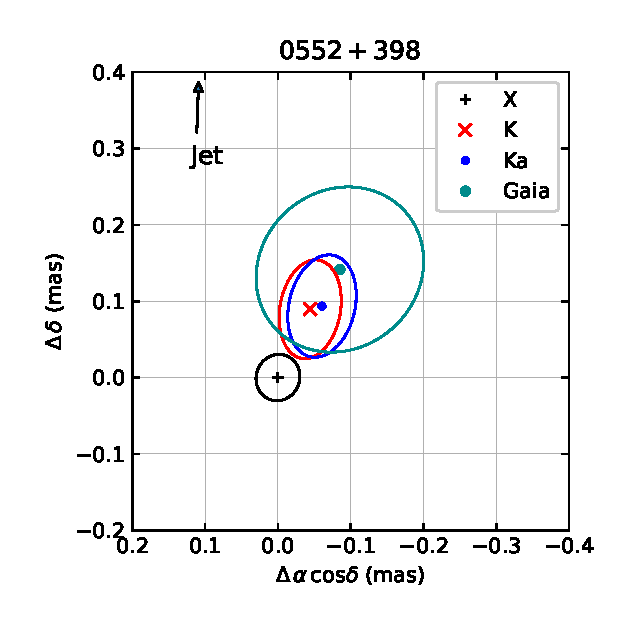
\includegraphics[width=70mm]{figs/0552+398}
        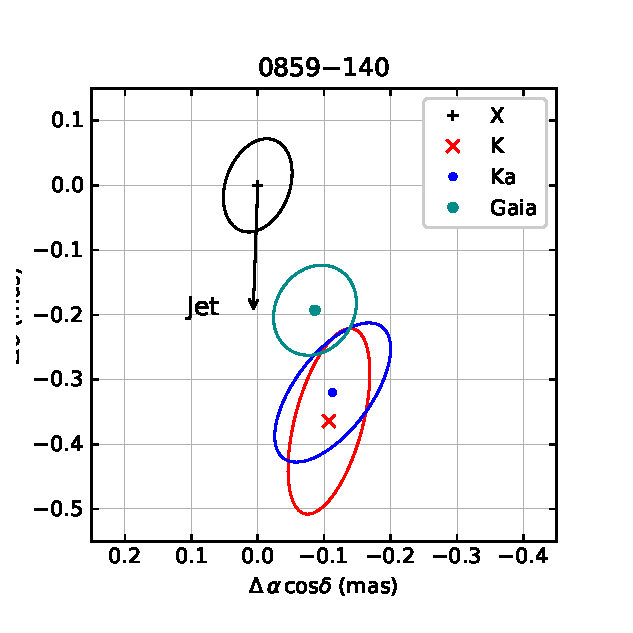
\includegraphics[width=70mm]{figs/0859-140}
        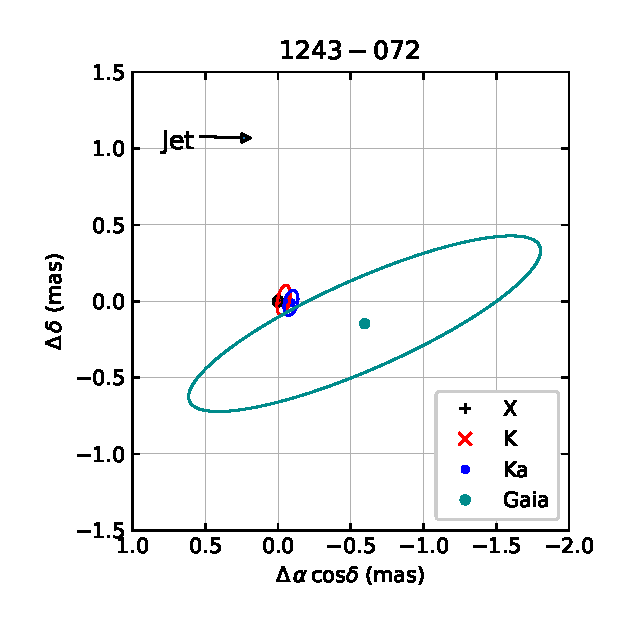
\includegraphics[width=70mm]{figs/1243-072}
        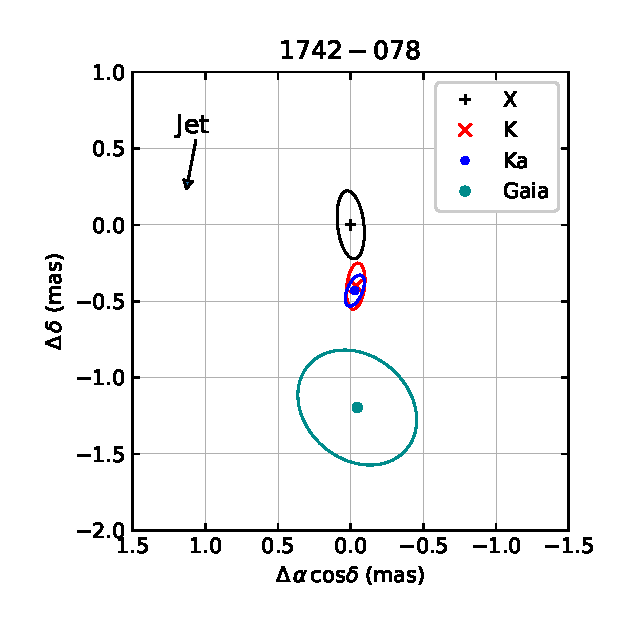
\includegraphics[width=70mm]{figs/1742-078}
        \includegraphics[width=70mm]{figs/2134+004}
        \caption[]{\label{fig:jet-down}
            Offset vectors of $K$-band, $Ka$-band, and {\it Gaia} (optical) positions with respect to the $X$-band position for sources with four position aligned as in the jet downstream.
            Also shown is the jet direction for these sources taken from MOJAVE database whilst the magnitude (length) is arbitrary and thus meaningless.
        }
    \end{figure*}

    %%
    %__________________________________________________{fig:fig:jet-up}

    \begin{figure*}[hbtp]
        \centering
        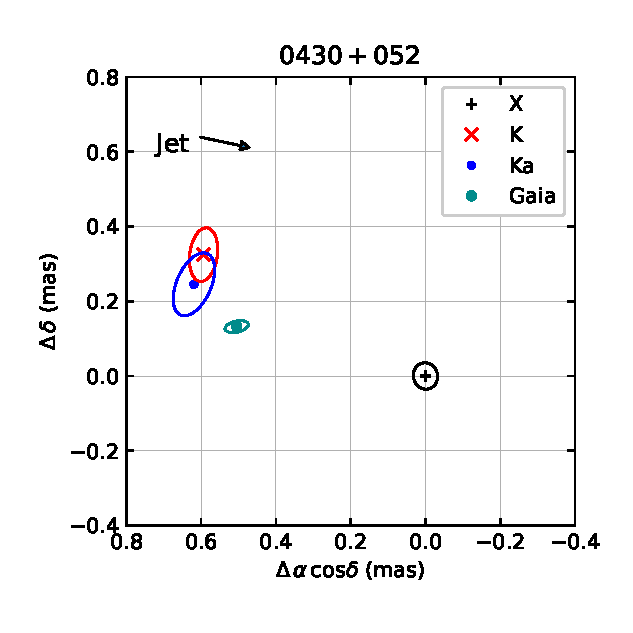
\includegraphics[width=70mm]{figs/0430+052}
        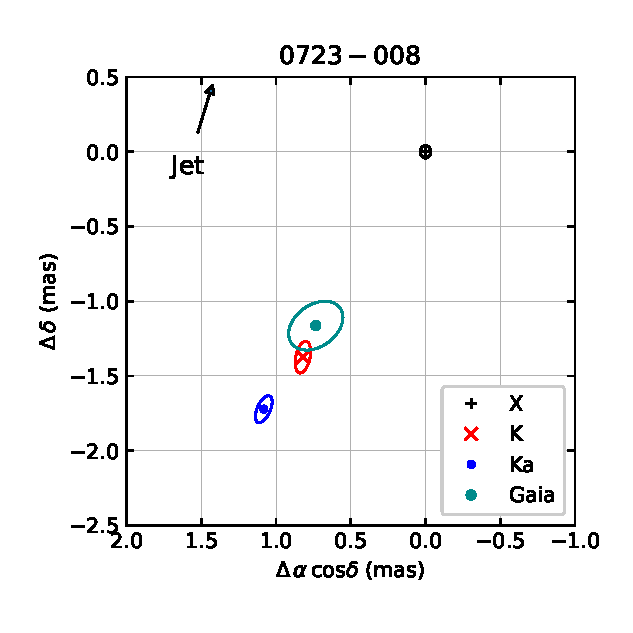
\includegraphics[width=70mm]{figs/0723-008}
        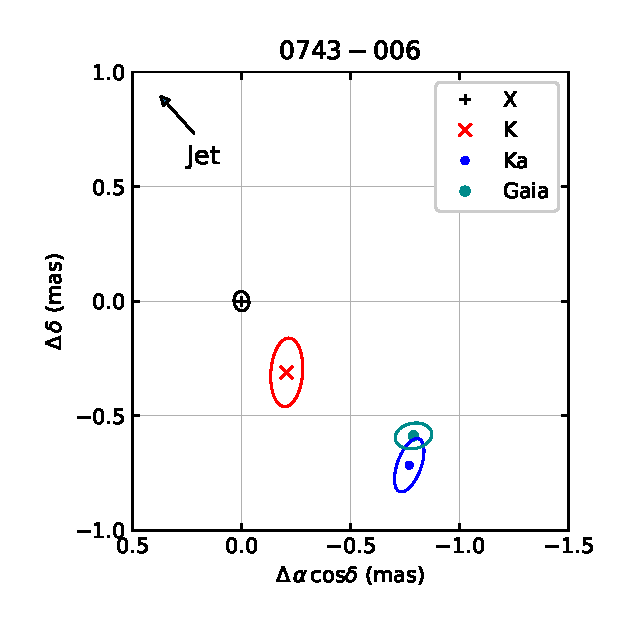
\includegraphics[width=70mm]{figs/0743-006}
        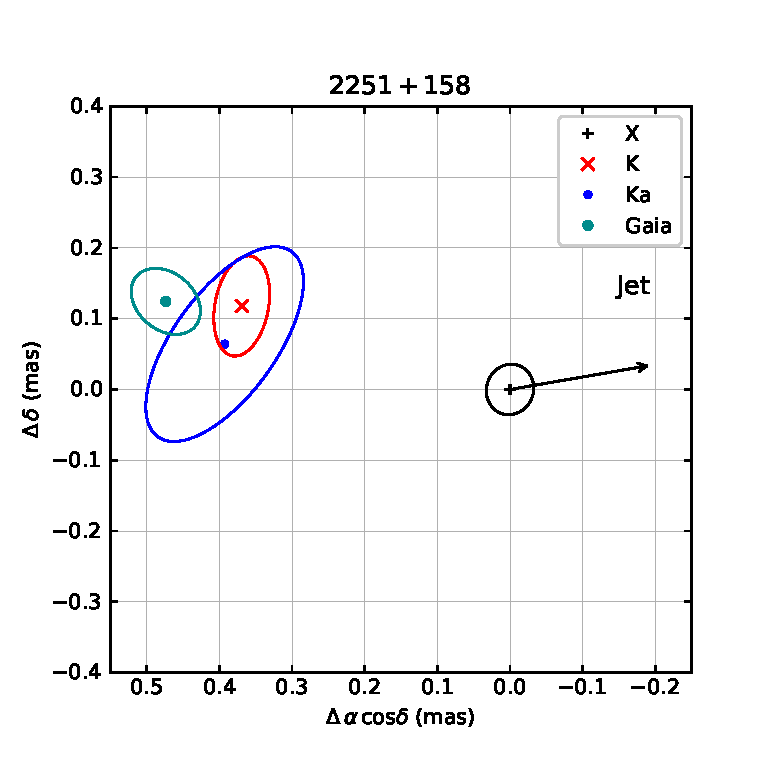
\includegraphics[width=70mm]{figs/2251+158}
        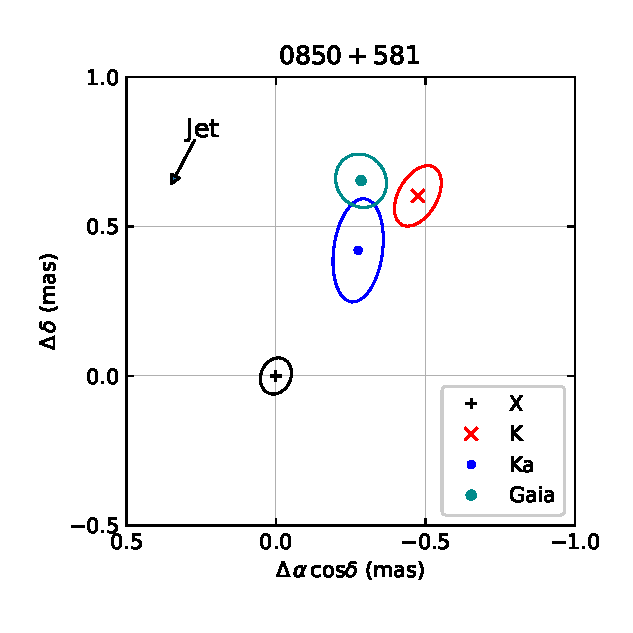
\includegraphics[width=70mm]{figs/0850+581}
        \caption[]{\label{fig:up}
            Offset vectors of $K$-band, $Ka$-band, and {\it Gaia} (optical) positions with respect to the $X$-band position for sources with four position aligned as in the jet upstream.
            Also shown is the jet direction for these sources taken from MOJAVE database whilst the magnitude (length) is arbitrary and thus meaningless.
        }
    \end{figure*}

    %%
    %__________________________________________________{fig:fig:jet-up}

    \begin{figure*}[hbtp]
        \centering
        \includegraphics[width=0.3\columnwidth]{figs/0003+380}
        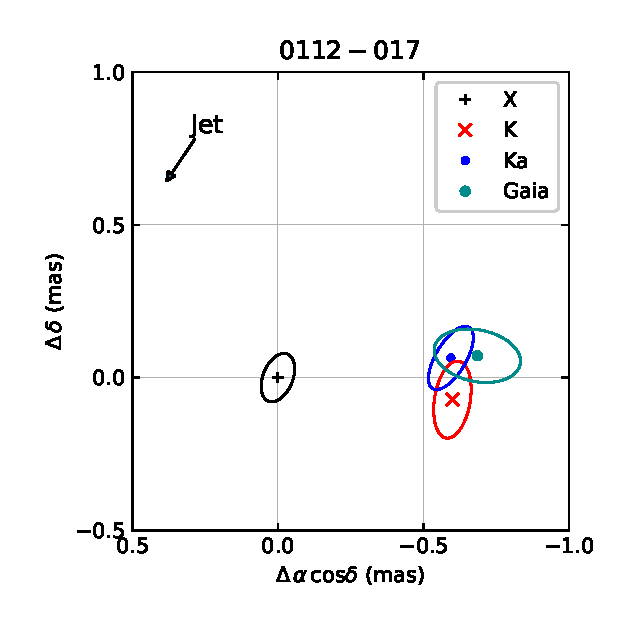
\includegraphics[width=0.3\columnwidth]{figs/0112-017}
        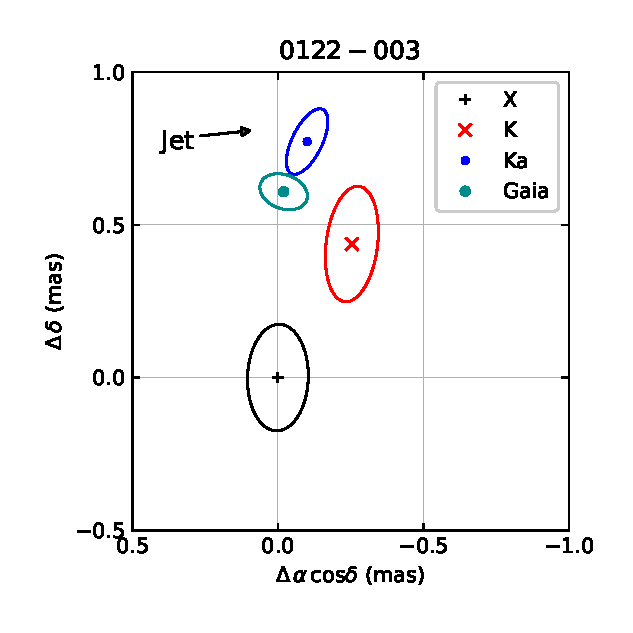
\includegraphics[width=0.3\columnwidth]{figs/0122-003}
        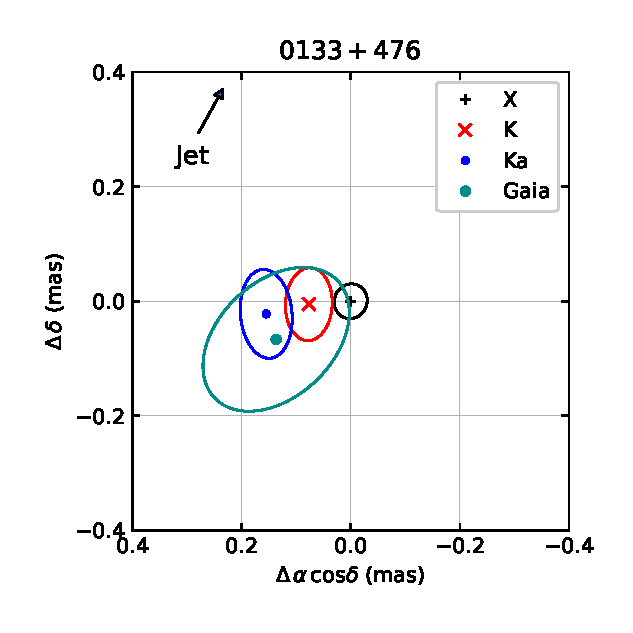
\includegraphics[width=0.3\columnwidth]{figs/0133+476}
        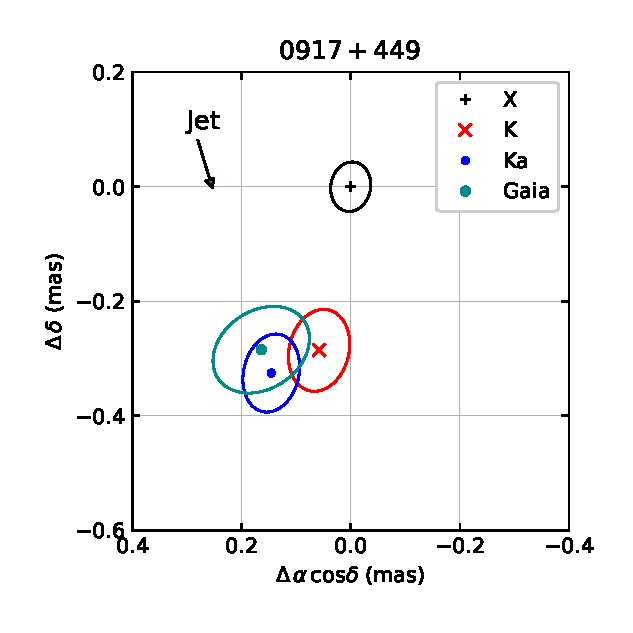
\includegraphics[width=0.3\columnwidth]{figs/0917+449}
        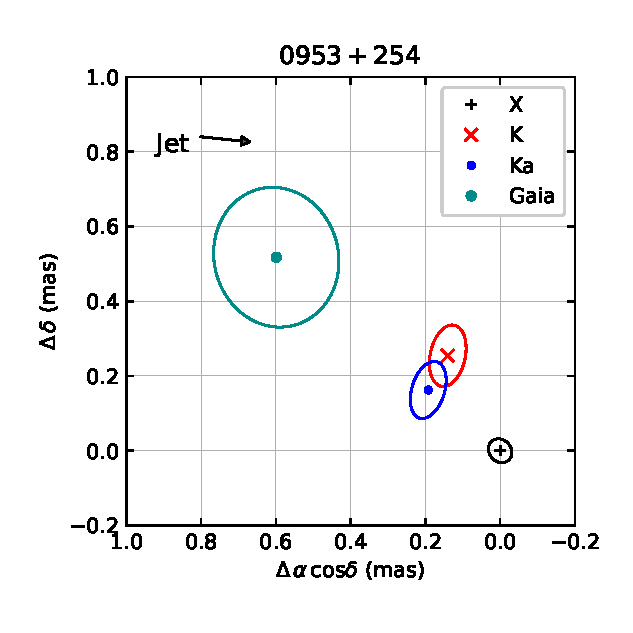
\includegraphics[width=0.3\columnwidth]{figs/0953+254}
        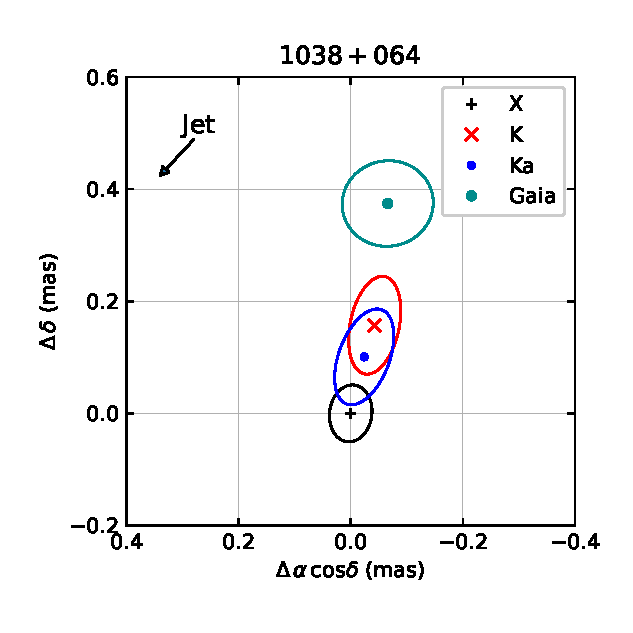
\includegraphics[width=0.3\columnwidth]{figs/1038+064}
        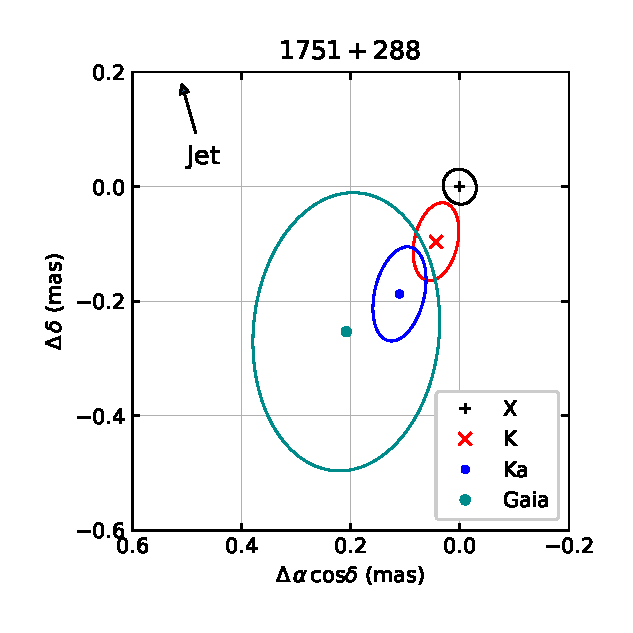
\includegraphics[width=0.3\columnwidth]{figs/1751+288}
        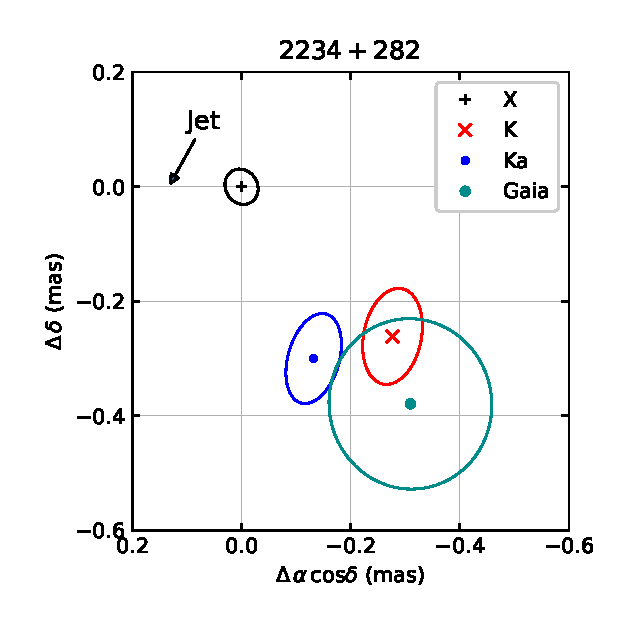
\includegraphics[width=0.3\columnwidth]{figs/2234+282}
        \caption[]{\label{fig:up}
            Offset vectors of $K$-band, $Ka$-band, and {\it Gaia} (optical) positions with respect to the $X$-band position for sources with four position aligned but not parallel to the jet direction.
            Also shown is the jet direction for these sources taken from MOJAVE database whilst the magnitude (length) is arbitrary and thus meaningless.
        }
    \end{figure*}

%__________________________________________________

%\section{Position simulation} \label{app:sim}
%We use the source 0838+45 to exemplify the process of simulation.
%We first computed three parameters of the error ellipse: semi-major axis $M$, semi-minor axis $m$, and the direction of semi-major axis $\theta$.
%Then we created coordinates of 10000 points, whose two components obey zero-mean Gaussian distributions with a standard deviation  of $M$ and $m$, respectively.
%These coordinates were rotated by the angle $\theta$ to get perturbed offsets ($\Delta\alpha^*$, $\Delta\delta$) to the original coordinates in the catalogs.
%These procedures were performed to all four catalogs, as shown in Fig.~\ref{fig:sim-pos}.
%The $Ka$-band position error ellipse elongate nearly along the declination axis.
%Then we calculate the $K$-to-$X$, $Ka$-to-$X$, and \textit{Gaia}-to-$X$ vectors and determined their distance and position angles.
%The scatter of $Ka$-to-$X$ vector is severely distorted by the asymmetry $Ka$-band uncertainty.
%Even at the $X$-band and \textit{Gaia} where the formal uncertainties on the right ascension and declination is at similar level, the peaks in the distance and PA of simulated samples do not match well with those calculated from the given positions.
%
%%__________________________________________________{fig:sim-pos}
%
%\begin{figure}[hbtp]
%    \centering
%    \includegraphics[width=0.48\columnwidth]{figs/0838+456-sim-x.png}
%    \includegraphics[width=0.48\columnwidth]{figs/0838+456-sim-k.png}
%    \includegraphics[width=0.48\columnwidth]{figs/0838+456-sim-ka.png}
%    \includegraphics[width=0.48\columnwidth]{figs/0838+456-sim-gaia.png}
%    \caption[]{\label{fig:sim-pos}
%        Simulation of the error ellipse for $X$- (top left), $K$- (top right), $Ka$-band (bottom left), and \textit{Gaia} (bottom right) positions for 0838+456.
%        The red, blue, and green circles indicates the interval of 1-$\sigma$, 2-$\sigma$, and 3-$\sigma$, respectively.
%    }
%\end{figure}

%__________________________________________________{fig:sim-pos-oft}

%\begin{figure}[hbtp]
%    \centering
%    \includegraphics[width=0.48\columnwidth]{figs/0838+456-sim-k-x.png}
%    \includegraphics[width=0.48\columnwidth]{figs/0838+456-sim-k-x-oft.png}
%    \includegraphics[width=0.48\columnwidth]{figs/0838+456-sim-ka-x.png}
%    \includegraphics[width=0.48\columnwidth]{figs/0838+456-sim-ka-x-oft.png}
%    \includegraphics[width=0.48\columnwidth]{figs/0838+456-sim-g-x.png}
%    \includegraphics[width=0.48\columnwidth]{figs/0838+456-sim-g-x-oft.png}
%    \caption[]{\label{fig:sim-pos-oft}
%        Left: Offset vectors of $K$-band, $Ka$-band, and {\it Gaia} (from top tp bottom) positions with respect to the $X$-band position for 0838+456.
%        Right: Distributions of distances and position angles of $K$-to-$X$, $Ka$-to-$X$, and \textit{Gaia}-to-$X$ vectors from 10\,000 simulated samples.
%        The red and blue vertical lines indicates the original and simulated values for distances and position angle.
%    }
%\end{figure}
%

\end{appendix}




\end{document}
